\chapter{Descrierea Modelului Ales și a Obiectivelor Aplicației}
\label{sec:descriere}

\section{Modelul de date ales}

TickLy este un sistem de management al tichetelor de suport care permite gestionarea a cererilor de asistență de la clienți. Modelul de date ales este un \textbf{model entitate-relație} extins care suportă atât clienți persoane fizice, cât și juridice, cu un sistem flexibil de categorisire și urmărire a tichetelor.

Sistemul este organizat în două straturi principale:
\begin{itemize}
    \item \textbf{Baza de date OLTP} - pentru operațiunile transacționale zilnice (creare tichete, comentarii, asignări agenți)
    \item \textbf{Data Warehouse} - pentru analize și raportare (model stea pentru analize multidimensionale)
\end{itemize}

\section{Obiectivele Aplicației}

Obiectivele principale ale aplicației TickLy sunt:

\begin{enumerate}
    \item \textbf{Gestionarea a tichetelor de suport} - urmărirea completă a ciclului de viață al tichetelor de la creare până la rezolvare
    \item \textbf{Analiza performanțelor agenților} - monitorizarea timpului de rezolvare, numărul de tichete rezolvate, rating-urile primite
    \item \textbf{Analiza satisfacției clienților} - urmărirea feedback-ului și identificarea tendințelor
    \item \textbf{Optimizare} - analiza distribuției tichetelor pe departamente și agenți
    \item \textbf{Identificarea problemelor recurente} - analiza categoriilor și subiectelor pentru a identifica problemele cele mai frecvente
    \item \textbf{Raportare} - generarea de rapoarte pentru management
\end{enumerate}

\chapter{Diagramele Bazei de Date OLTP}
\label{sec:diagrame_oltp}

\section{Diagrama Entitate-Relație}
\label{subsec:er_diagram}

Diagrama entitate-relație a bazei de date OLTP este prezentată mai jos:
\begin{figure}[H]
    \centering
    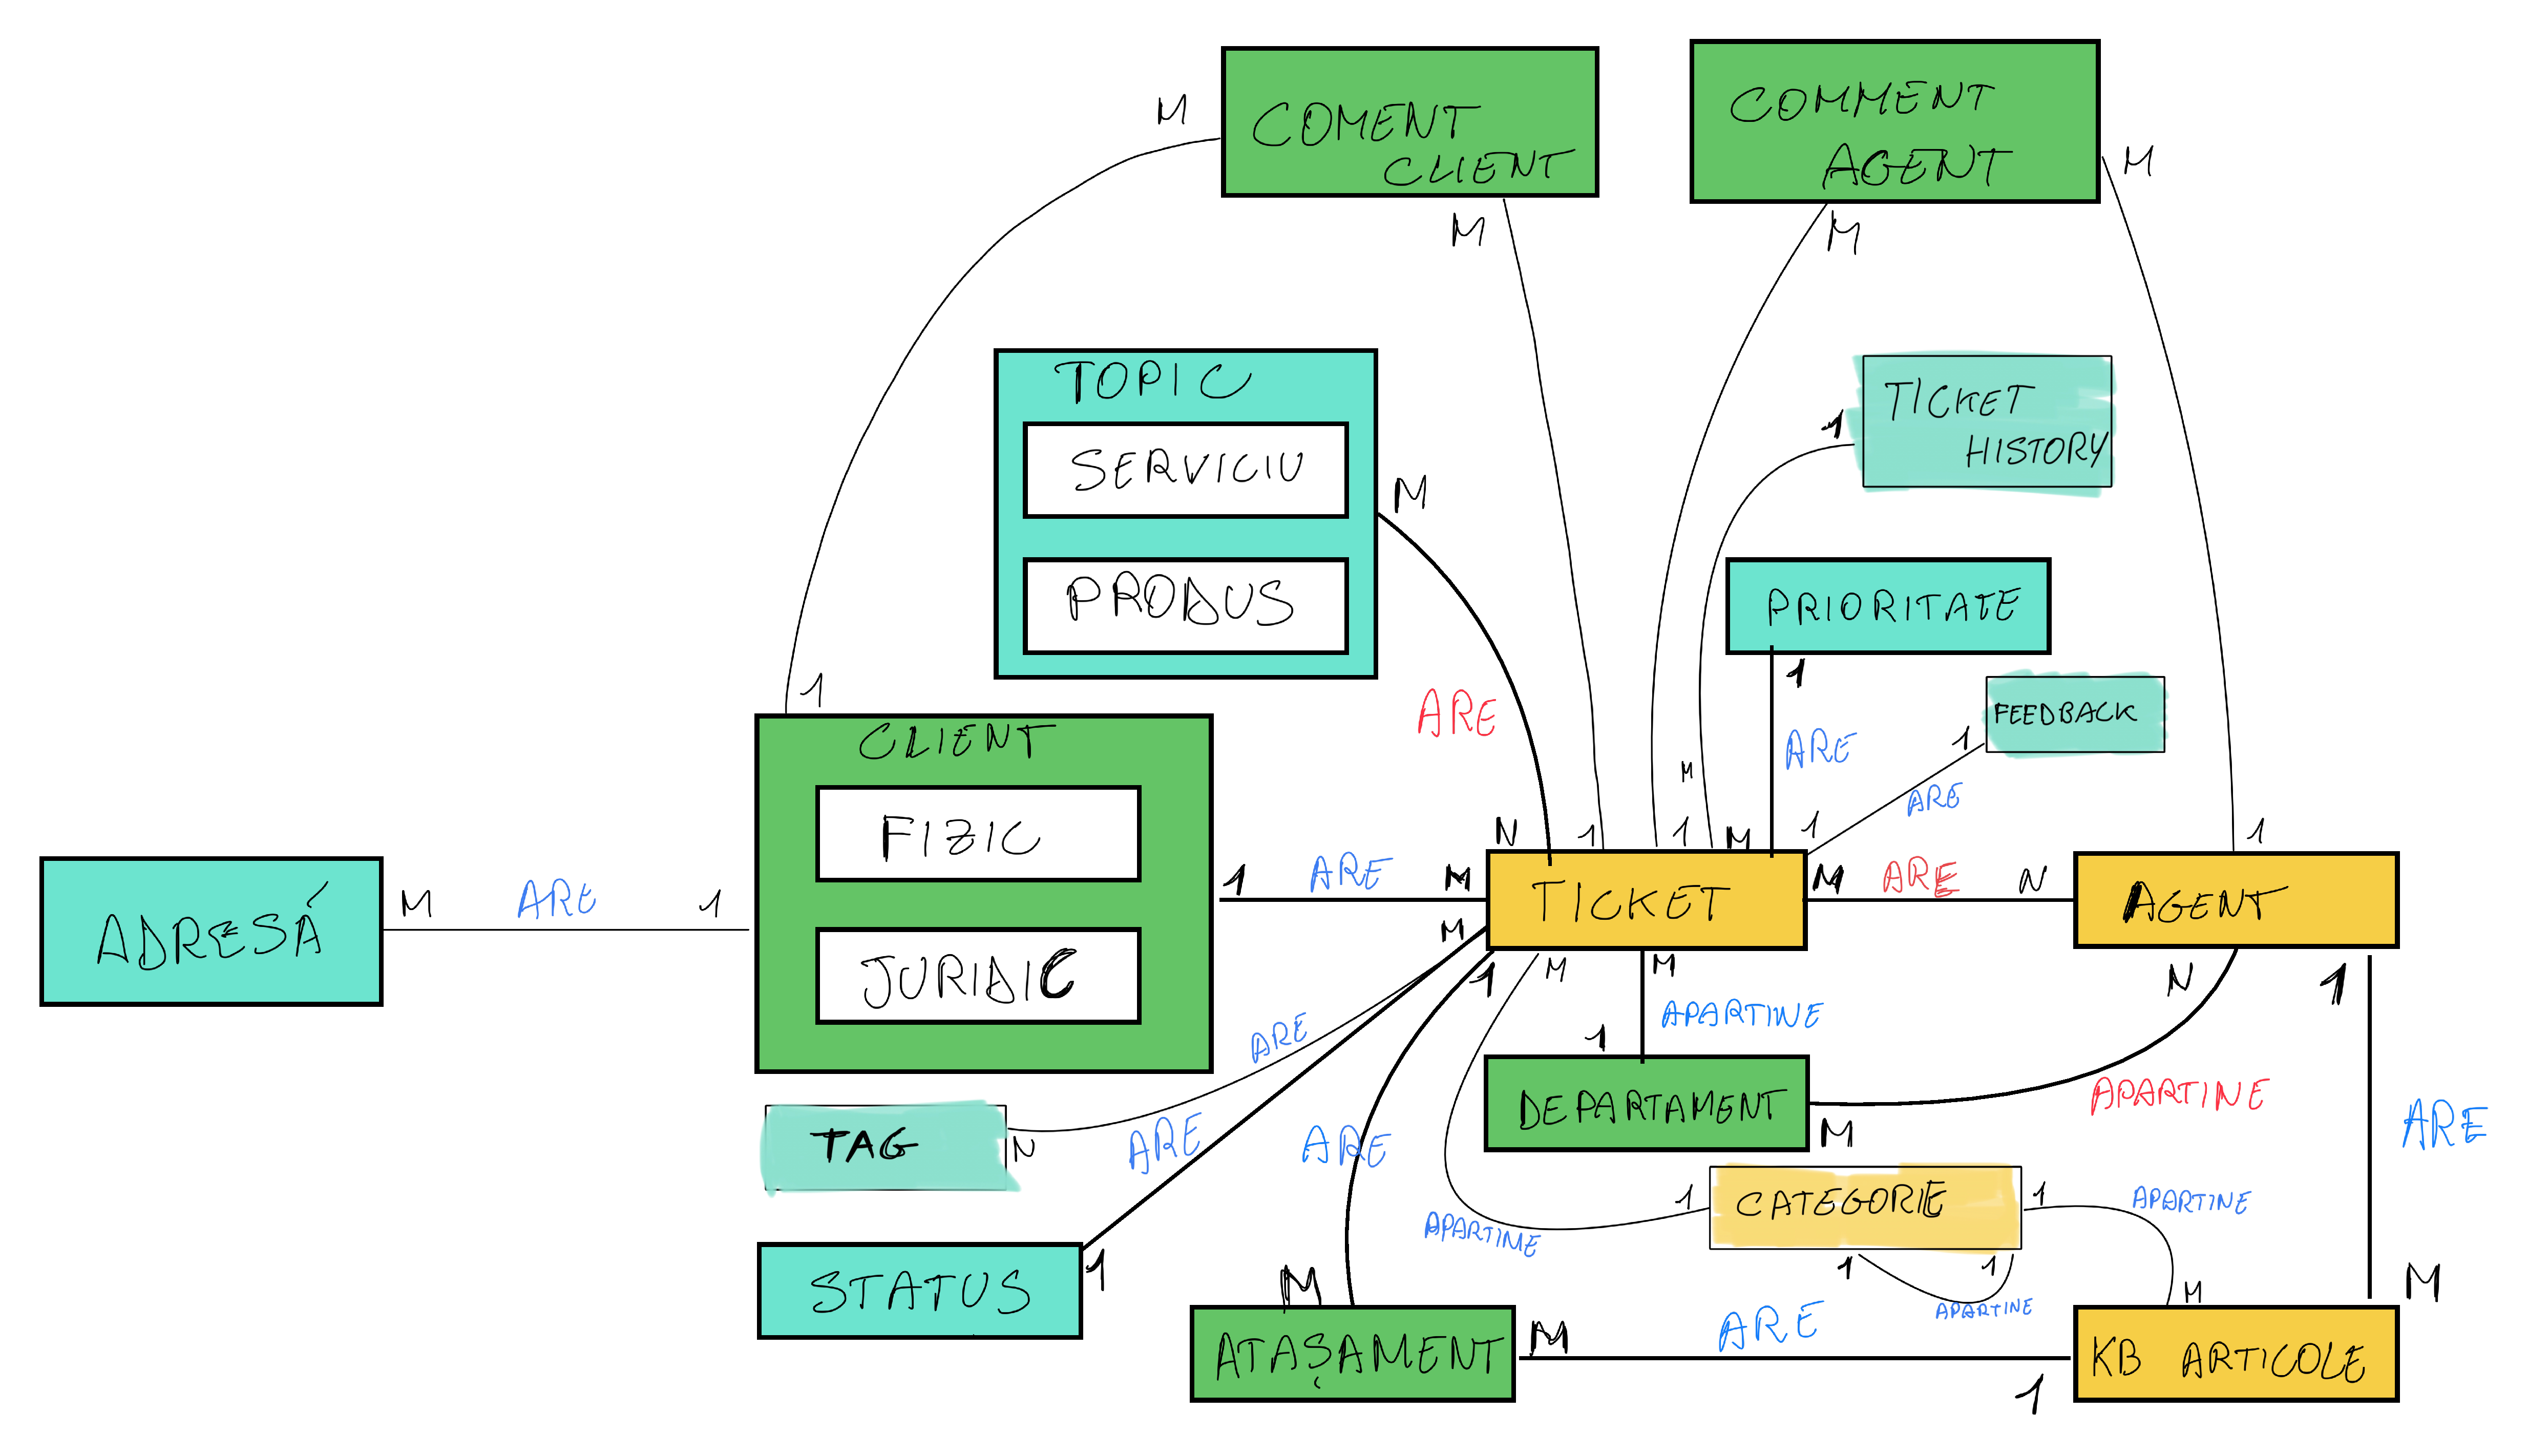
\includegraphics[width=1.0\textwidth]{../../schema/TickLy ER Diagram_Initiala.pdf}
    \caption{Diagrama Entitate-Relație a Bazei de Date OLTP}
    \label{fig:er_diagram}
\end{figure}

Această diagramă prezintă:
\begin{itemize}
    \item Toate entitățile
    \item Relațiile între entități (1:1, 1:M, M:N)
\end{itemize}

\section{Diagrama Conceptuală Extinsă}
\label{subsec:conceptual_diagram}

Diagrama conceptuală extinsă a bazei de date OLTP este prezentată mai jos:
\begin{figure}[H]
    \centering
    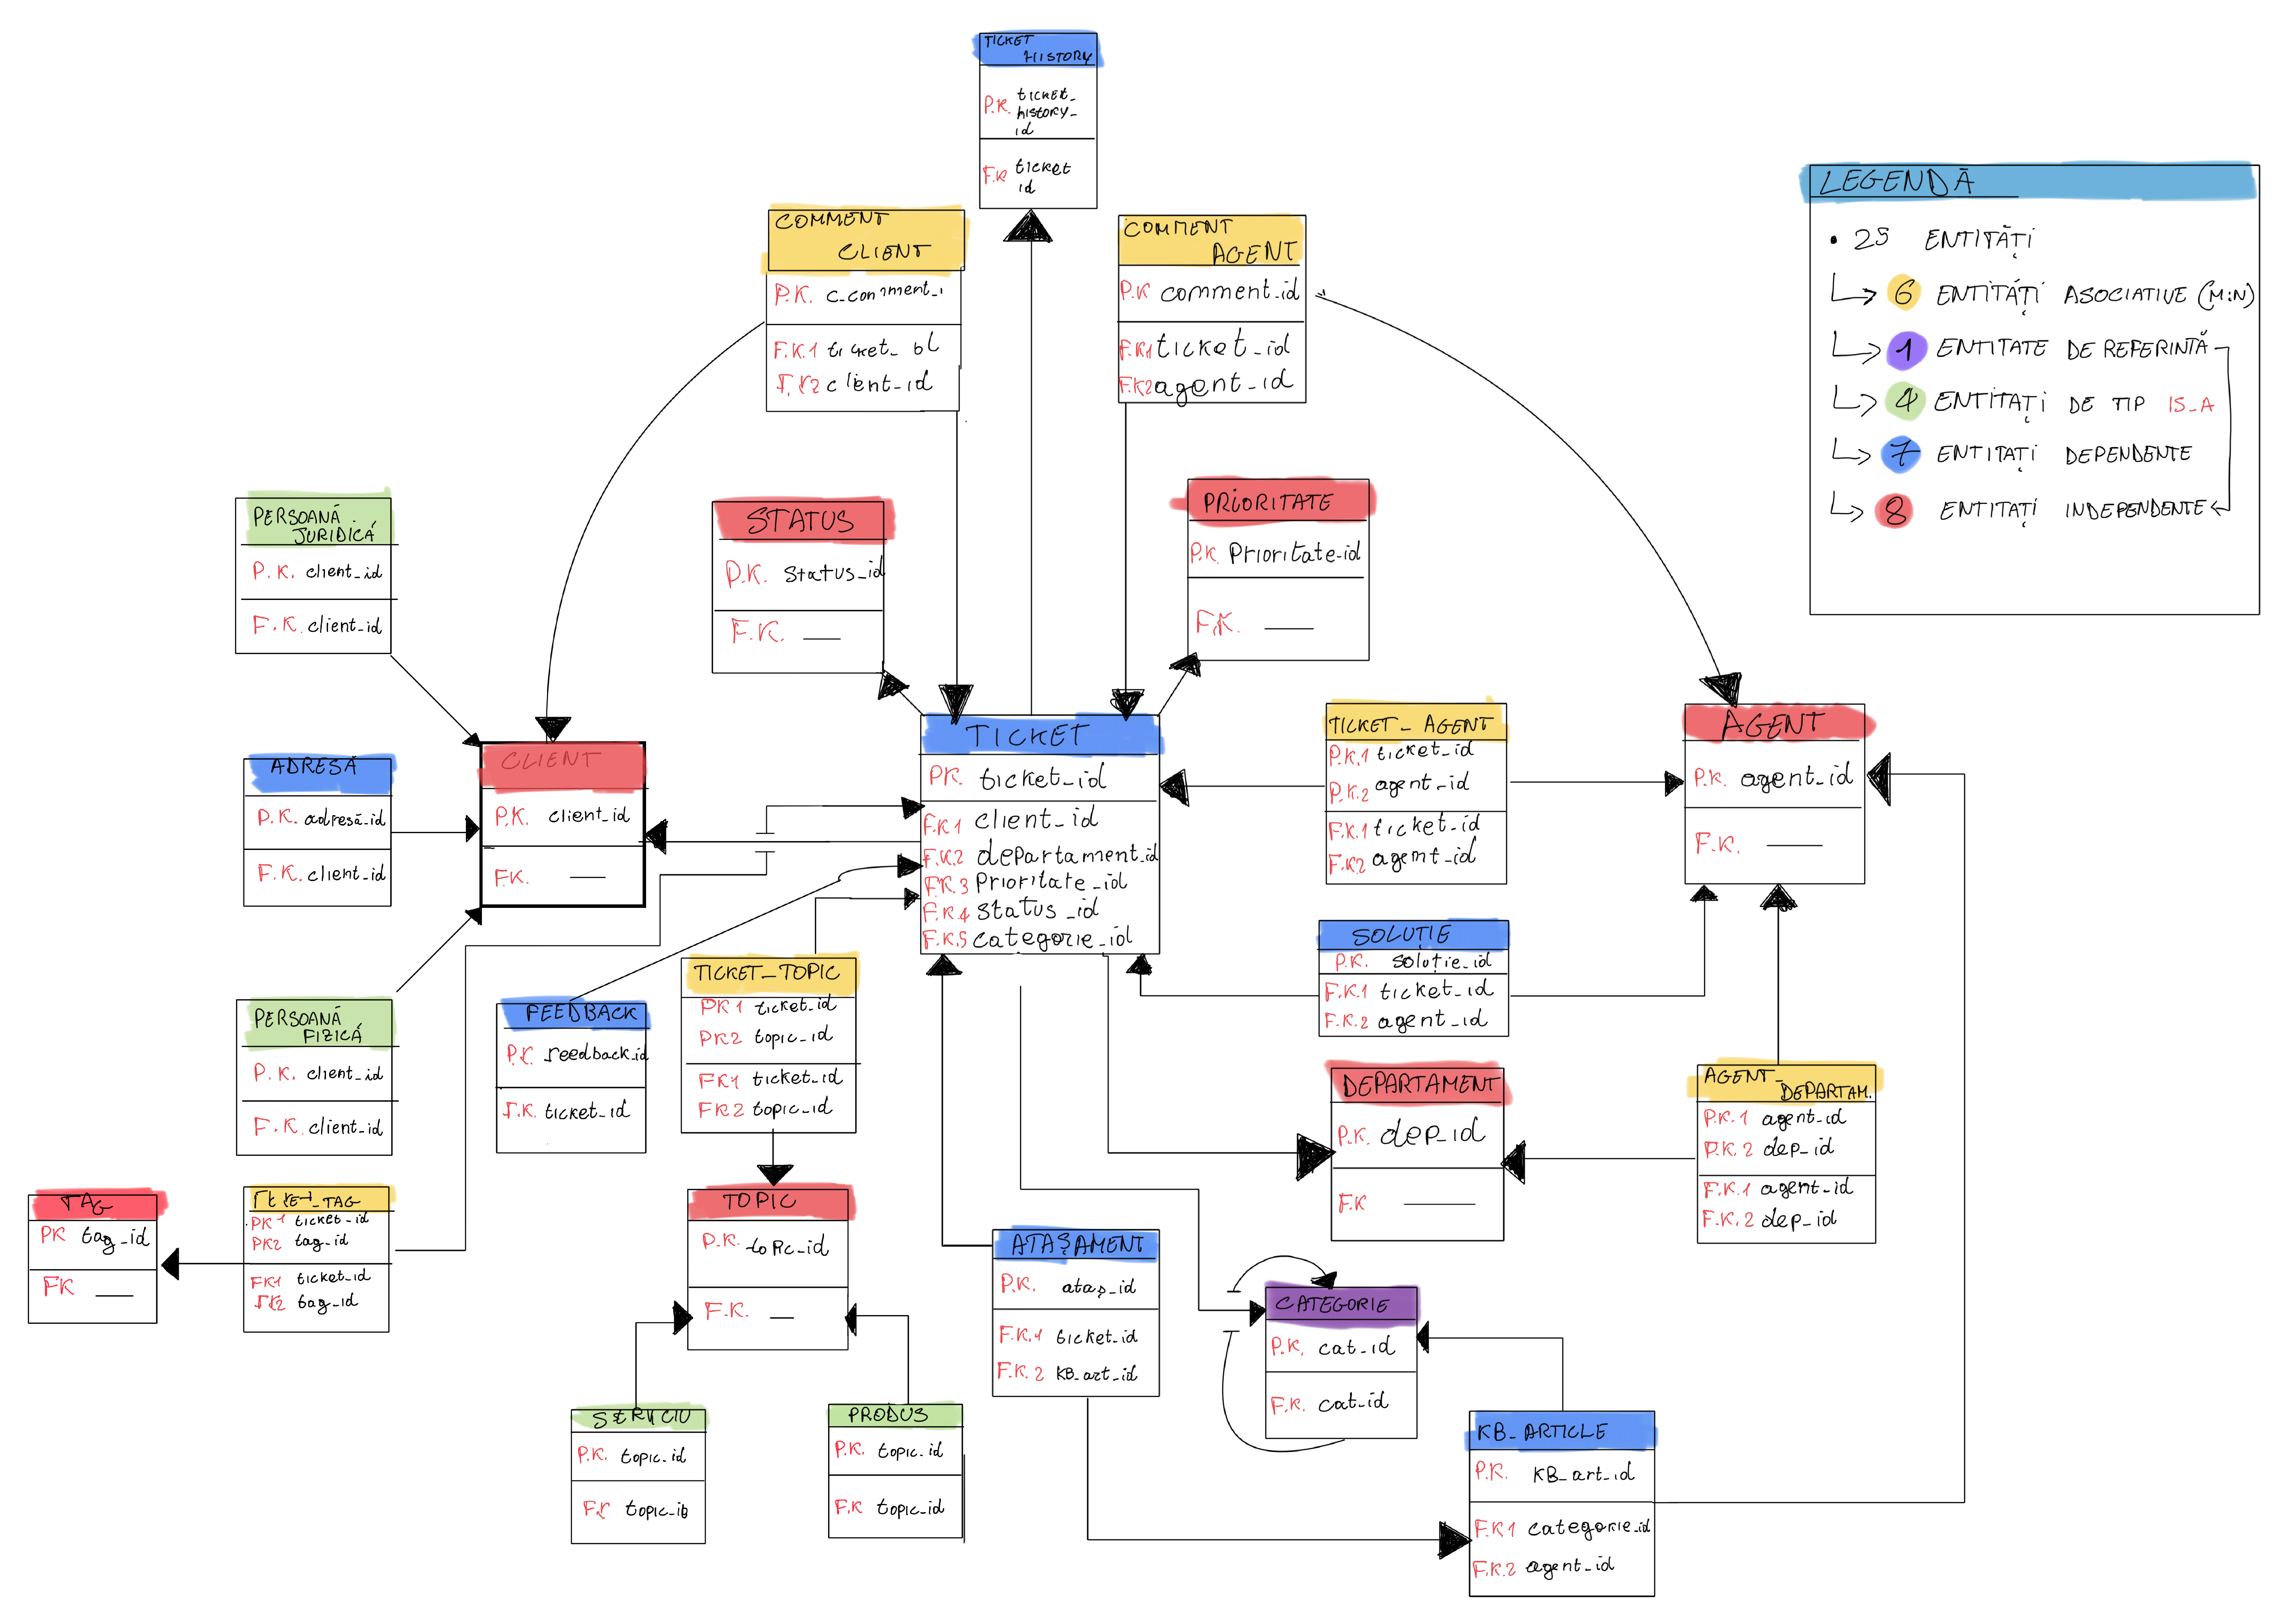
\includegraphics[width=1.0\textwidth]{../../schema/TickLy Conceptuală Extinsă.pdf}
    \caption{Diagrama Conceptuală Extinsă a Bazei de Date OLTP}
    \label{fig:conceptual_diagram}
\end{figure}

Baza de date OLTP conține următoarele: 

\subsubsection{Entități independente}

\begin{enumerate}
    \item \textbf{CLIENT} — entitate părinte pentru clienți
    \item \textbf{AGENT} — agenții de suport
    \item \textbf{PRIORITATE} — nivelurile de prioritate ale tichetelor
    \item \textbf{STATUS} — statusurile tichetelor
    \item \textbf{TOPIC} — entitate părinte pentru topic-urile asociate tichetelor
    \item \textbf{CATEGORIE} — categoriile pentru organizarea tichetelor
    \item \textbf{TAG} — tag-uri pentru etichetarea tichetelor
    \item \textbf{DEPARTAMENT} — departamentele organizației
\end{enumerate}

\textbf{Nota:} Categorie este o entitate de referinta catre categoria parinte.

\subsubsection{Entități dependente}

\begin{enumerate}
    \item \textbf{TICKET} — tichetele de suport
    \item \textbf{TICKET\_HISTORY} — istoricul evenimentelor pe tichete (audit trail)
    \item \textbf{ATASAMENT} — atașamentele la tichete sau la articole KB
    \item \textbf{KB\_ARTICLE} — articole din baza de cunoștințe (documentație)
    \item \textbf{FEEDBACK} — feedback-urile clienților la tichete (rating, comentariu)
    \item \textbf{SOLUTIE} — soluțiile înregistrate la tichete rezolvate
    \item \textbf{ADRESA} — adresele clienților (facturare, livrare, sediu)
\end{enumerate}

\subsubsection{Entități de tip IS-A}

\begin{enumerate}
    \item \textbf{CLIENT $\rightarrow$ CLIENT\_FIZICA / CLIENT\_JURIDICA} — clienți persoane fizice sau juridice
    \item \textbf{TOPIC $\rightarrow$ TOPIC\_SERVICIU / TOPIC\_PRODUS} — topic-uri de tip serviciu sau produs
\end{enumerate}

\subsubsection{Relații Many-to-Many}

Sistemul conține următoarele relații many-to-many (M:N), implementate prin tabele asociative:

\begin{itemize}
    \item \textbf{Ticket $\leftrightarrow$ Agent} (prin \texttt{TICKET\_AGENT}) - un ticket poate fi asignat mai multor agenți, iar un agent poate lucra la mai multe tichete
    \item \textbf{Ticket $\leftrightarrow$ Topic} (prin \texttt{TICKET\_TOPIC}) - un ticket poate fi asociat cu mai multe topic-uri, iar un topic poate fi asociat cu mai multe tichete
    \item \textbf{Agent $\leftrightarrow$ Departament} (prin \texttt{AGENT\_DEPARTAMENT}) - un agent poate aparține mai multor departamente, iar un departament poate avea mai mulți agenți
    \item \textbf{Ticket $\leftrightarrow$ Tag} (prin \texttt{TICKET\_TAG}) - un ticket poate avea mai multe tag-uri, iar un tag poate fi asociat cu mai multe tichete
    \item \textbf{Comment $\leftrightarrow$ Client} (prin \texttt{COMMENT\_CLIENT}) - un ticket poate avea mai multe comentarii de la client, iar un client poate avea mai multe comentarii la tichete
    \item \textbf{Comment $\leftrightarrow$ Agent} (prin \texttt{COMMENT\_AGENT}) - un ticket poate avea mai multe comentarii de la agent, iar un agent poate avea mai multe comentarii la tichete
\end{itemize}

\chapter{Diagrama Stea/Fulg a Bazei de Date Depozit}
\label{sec:diagrama_stea}

\begin{figure}[H]
    \centering
    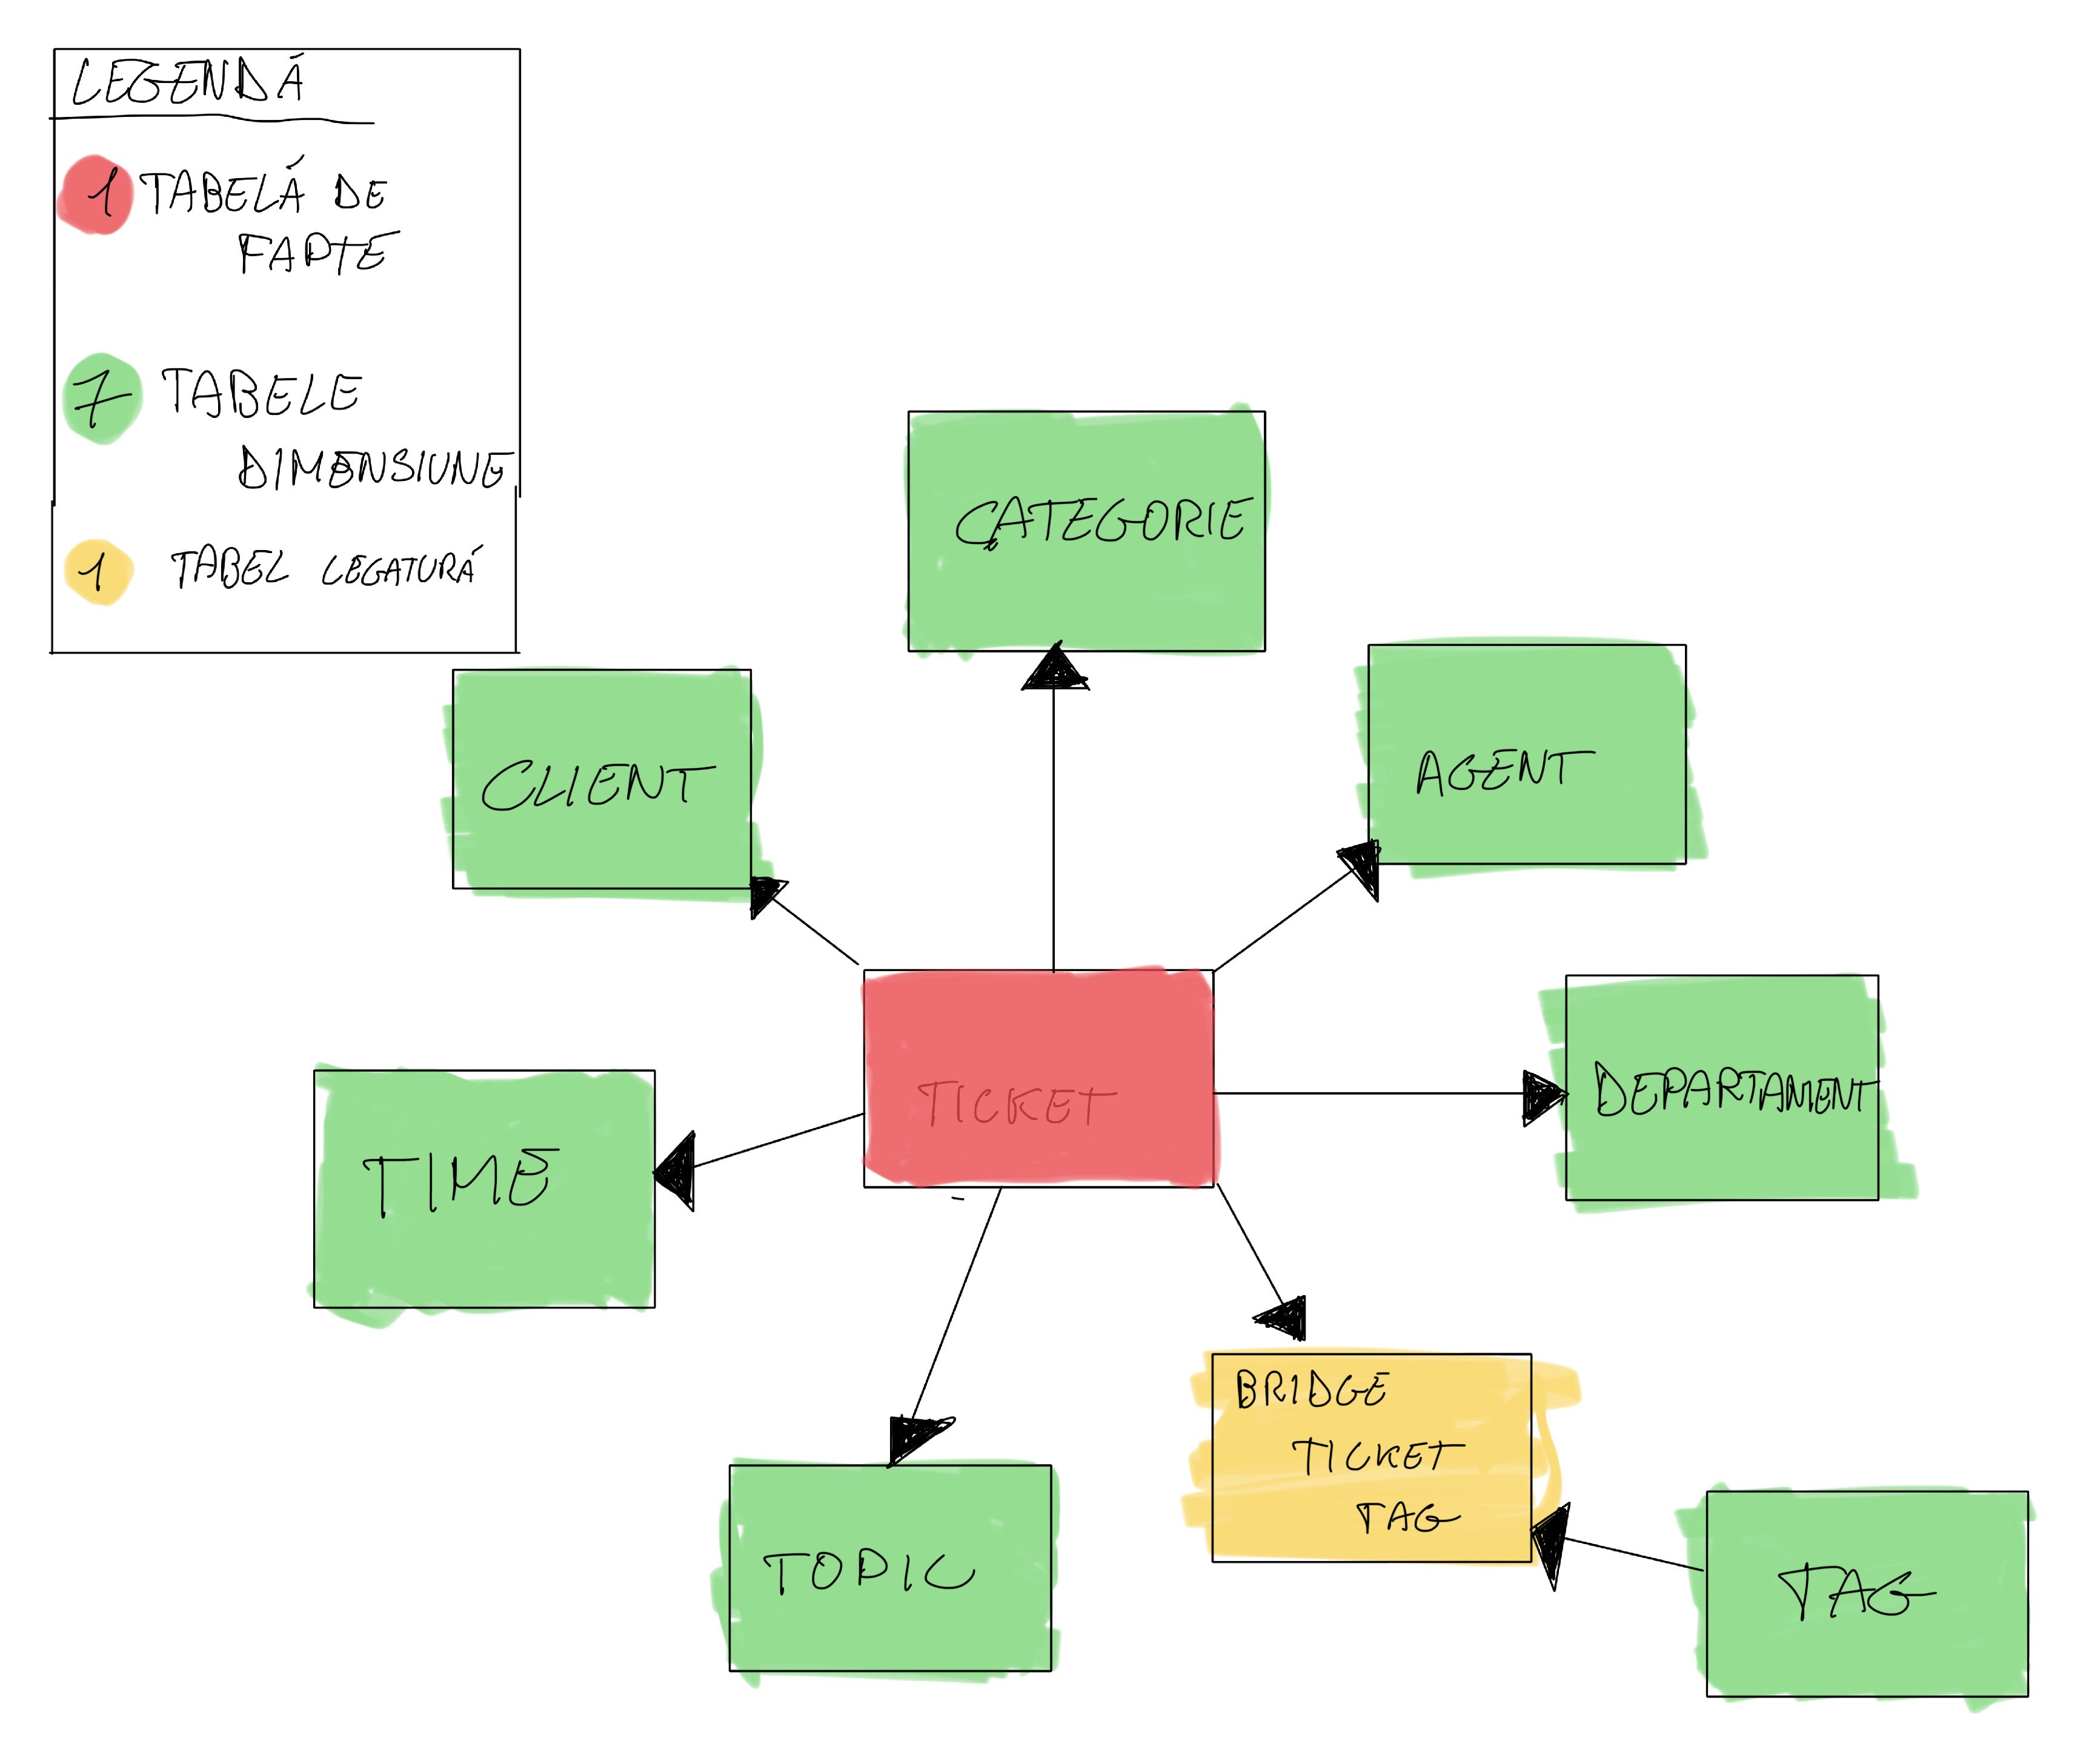
\includegraphics[width=1.0\textwidth]{../../schema/TickLy Schema Stea Simplificata.pdf}
    \caption{Diagrama Stea a Bazei de Date Depozit}
    \label{fig:stea_diagram}
\end{figure}

\section{Structura Modelului Stea}

Modelul stea implementat pentru TickLy conține:

\subsubsection{Tabel de Fapte}

\begin{itemize}
    \item \textbf{FACT\_TICKET} — tabelul central de fapte care stochează măsurile și metricile asociate tichetelor (chei către dimensiuni, status, prioritate, cost estimativ, timp rezolvare)
\end{itemize}

\subsubsection{Tabel de Legătură (Bridge)}

\begin{itemize}
    \item \textbf{BRIDGE\_TICKET\_TAG} — tabel de legătură many-to-many între \texttt{FACT\_TICKET} și \texttt{DIM\_TAG}; permite asocierea mai multor tag-uri la un ticket, cu \texttt{weight\_factor} (ex. 1 / număr tag-uri per ticket)
\end{itemize}

\subsubsection{Tabele Dimensiune}

\begin{enumerate}
    \item \textbf{DIM\_CLIENT} - dimensiunea clienților (Type 2 SCD pentru istoricizare)
    \item \textbf{DIM\_AGENT} - dimensiunea agenților (Type 2 SCD)
    \item \textbf{DIM\_DEPARTAMENT} - dimensiunea departamentelor (Type 2 SCD)
    \item \textbf{DIM\_CATEGORIE} - dimensiunea categoriilor (Type 1 SCD)
    \item \textbf{DIM\_TOPIC} - dimensiunea topic-urilor (Type 1 SCD)
    \item \textbf{DIM\_TAG} - dimensiunea tag-urilor (Type 1 SCD)
    \item \textbf{DIM\_TIME} - dimensiunea temporală pentru analize pe perioade
\end{enumerate}

\begin{itemize}
    \item \textbf{Nota - Type 1 SCD:} nu permite urmărirea istoricului modificărilor.
    \item \textbf{Nota - Type 2 SCD:} permite urmărirea istoricului modificărilor.
\end{itemize}

\section{Caracteristici ale Modelului}

\begin{itemize}
    \item \textbf{Slowly Changing Dimensions (SCD)}: Dimensiunile \texttt{DIM\_CLIENT}, \texttt{DIM\_AGENT} și \texttt{DIM\_DEPARTAMENT} sunt implementate ca Type 2 SCD, permițând urmărirea istoricului modificărilor
    \item \textbf{Degenerări}: Status și Prioritate sunt degenerate în tabelul de fapte (stocate direct în \texttt{FACT\_TICKET})
    \item \textbf{Dimensiune Conformată}: Dimensiunea temporală \texttt{DIM\_TIME}
\end{itemize}

\chapter{Descrierea Câmpurilor și Modul de Populare}
\label{sec:campuri_populare}

\section{Tabelul de Fapte: FACT\_TICKET}

\subsubsection{Câmpuri și Sursa de Date}

\begin{longtable}{|>{\raggedright\arraybackslash}p{3.5cm}|>{\raggedright\arraybackslash}p{2.8cm}|>{\raggedright\arraybackslash}p{8.7cm}|}
\hline
\textbf{Câmp} & \textbf{Tip} & \textbf{Mod de Populare din OLTP} \\
\hline
\endfirsthead
\hline
\textbf{Câmp} & \textbf{Tip} & \textbf{Mod de Populare din OLTP} \\
\hline
\endhead
\hline
\endfoot
\hline
\endlastfoot

\texttt{fact\_ticket\_id} & NUMBER & Generat automat (IDENTITY) \\
\hline
\texttt{ticket\_id} & NUMBER & Copiat direct din \texttt{TICKET.ticket\_id} \\
\hline
\texttt{client\_key} & NUMBER & Lookup în \texttt{DIM\_CLIENT} pe baza \texttt{TICKET.client\_id} (\texttt{is\_current = 'Y'}) \\
\hline
\texttt{agent\_key} & NUMBER & Lookup în \texttt{DIM\_AGENT} pe baza \texttt{TICKET\_AGENT.agent\_id} (rol PRIMARY), fallback agent\_id = 1 \\
\hline
\texttt{departament\_key} & NUMBER & Lookup în \texttt{DIM\_DEPARTAMENT} pe baza \texttt{TICKET.departament\_id} (\texttt{is\_current = 'Y'}) \\
\hline
\texttt{categorie\_key} & NUMBER & Lookup în \texttt{DIM\_CATEGORIE} pe baza \texttt{TICKET.categorie\_id} (poate fi NULL) \\
\hline
\texttt{topic\_key} & NUMBER & Lookup în \texttt{DIM\_TOPIC} pe baza \texttt{TICKET\_TOPIC} (MIN(topic\_id) per ticket) \\
\hline
\ttwrap{date\_creare\_key} & NUMBER & \texttt{TO\_NUMBER(TO\_CHAR(TICKET.data\_creare, 'YYYYMMDD'))} — lookup în \texttt{DIM\_TIME} \\
\hline
\ttwrap{date\_rezolvare\_key} & NUMBER & \texttt{TO\_NUMBER(TO\_CHAR(TICKET.data\_rezolvare, 'YYYYMMDD'))} (poate fi NULL) \\
\hline
\ttwrap{date\_inchidere\_key} & NUMBER & \texttt{TO\_NUMBER(TO\_CHAR(TICKET.data\_inchidere, 'YYYYMMDD'))} (poate fi NULL) \\
\hline
\texttt{status\_id} & NUMBER & Copiat din \texttt{TICKET} JOIN \texttt{STATUS} \\
\hline
\texttt{status\_nume} & VARCHAR2(30) & JOIN cu \texttt{STATUS.nume} \\
\hline
\ttwrap{status\_este\_final} & CHAR(1) & JOIN cu \texttt{STATUS.este\_final} \\
\hline
\texttt{prioritate\_id} & NUMBER & Copiat din \texttt{TICKET} JOIN \texttt{PRIORITATE} \\
\hline
\texttt{prioritate\_nume} & VARCHAR2(20) & JOIN cu \texttt{PRIORITATE.nume} \\
\hline
\texttt{cost\_estimativ} & NUMBER(10,2) & Din \texttt{DIM\_TOPIC.pret} (topic asociat ticketului) \\
\hline
\ttwrap{timp\_rezolvare\_ore} & NUMBER & Copiat din \texttt{TICKET.timp\_rezolvare\_ore} \\
\hline
\texttt{load\_date} & DATE & SYSDATE la momentul încărcării (ETL) \\
\hline
\end{longtable}

\section{Tabelul de Legătură: BRIDGE\_TICKET\_TAG}

\subsubsection{Câmpuri și Sursa de Date}

\begin{longtable}{|>{\raggedright\arraybackslash}p{3.5cm}|>{\raggedright\arraybackslash}p{2.8cm}|>{\raggedright\arraybackslash}p{8.7cm}|}
\hline
\textbf{Câmp} & \textbf{Tip} & \textbf{Mod de Populare din OLTP} \\
\hline
\endfirsthead
\hline
\textbf{Câmp} & \textbf{Tip} & \textbf{Mod de Populare din OLTP} \\
\hline
\endhead
\hline
\endfoot
\hline
\endlastfoot

\texttt{bridge\_id} & NUMBER & Generat automat (IDENTITY), cheie primară \\
\hline
\texttt{fact\_ticket\_id} & NUMBER & Lookup în \texttt{FACT\_TICKET} pe baza \texttt{TICKET\_TAG.ticket\_id} (JOIN \texttt{tt\_oltp.ticket\_id = f.ticket\_id}) \\
\hline
\texttt{tag\_key} & NUMBER & Lookup în \texttt{DIM\_TAG} pe baza \texttt{TICKET\_TAG.tag\_id} (JOIN \texttt{tt\_oltp.tag\_id = dt.tag\_id}) \\
\hline
\texttt{weight\_factor} & NUMBER & Calculat ca \texttt{1 / COUNT(*) OVER (PARTITION BY fact\_ticket\_id)} — distribuire uniformă a „greutății” pe tag-urile unui același ticket (suma weight\_factor pe ticket = 1) \\
\hline
\end{longtable}

\section{Dimensiunea: DIM\_CLIENT}

\begin{longtable}{|>{\raggedright\arraybackslash}p{3.5cm}|>{\raggedright\arraybackslash}p{2.8cm}|>{\raggedright\arraybackslash}p{8.7cm}|}
\hline
\textbf{Câmp} & \textbf{Tip} & \textbf{Mod de Populare din OLTP} \\
\hline
\endfirsthead
\hline
\textbf{Câmp} & \textbf{Tip} & \textbf{Mod de Populare din OLTP} \\
\hline
\endhead
\hline
\endfoot
\hline
\endlastfoot

\texttt{client\_key} & NUMBER & Generat automat (IDENTITY) \\
\hline
\texttt{client\_id} & NUMBER & Copiat din \texttt{CLIENT.client\_id} \\
\hline
\texttt{email} & VARCHAR2 & Copiat din \texttt{CLIENT.email} \\
\hline
\texttt{phone} & VARCHAR2 & Copiat din \texttt{CLIENT.phone} \\
\hline
\ttwrap{registration\_date} & DATE & Copiat din \texttt{CLIENT.registration\_date} \\
\hline
\texttt{client\_type} & CHAR(1) & Copiat din \texttt{CLIENT.client\_type} ('F' sau 'J') \\
\hline
\texttt{nume} & VARCHAR2 & Copiat din \texttt{CLIENT\_FIZICA.nume} (dacă \texttt{client\_type = 'F'}) \\
\hline
\texttt{prenume} & VARCHAR2 & Copiat din \texttt{CLIENT\_FIZICA.prenume} (dacă \texttt{client\_type = 'F'}) \\
\hline
\texttt{cnp} & VARCHAR2 & Copiat din \texttt{CLIENT\_FIZICA.cnp} (dacă \texttt{client\_type = 'F'}) \\
\hline
\texttt{denumire} & VARCHAR2 & Copiat din \texttt{CLIENT\_JURIDICA.denumire} (dacă \texttt{client\_type = 'J'}) \\
\hline
\texttt{cui} & VARCHAR2 & Copiat din \texttt{CLIENT\_JURIDICA.cui} (dacă \texttt{client\_type = 'J'}) \\
\hline
\texttt{sediu\_social} & VARCHAR2 & Copiat din \texttt{CLIENT\_JURIDICA.sediu\_social} (dacă \texttt{client\_type = 'J'}) \\
\hline
\ttwrap{reprezentant\_legal} & VARCHAR2 & Copiat din \texttt{CLIENT\_JURIDICA.reprezentant\_legal} (dacă \texttt{client\_type = 'J'}) \\
\hline
\texttt{is\_active} & CHAR(1) & Calculat pe baza existenței tichetelor recente sau flag explicit \\
\hline
\texttt{valid\_from} & DATE & SYSDATE pentru înregistrări noi, sau data modificării pentru SCD Type 2 \\
\hline
\texttt{valid\_to} & DATE & NULL pentru înregistrări curente, sau data modificării pentru înregistrări istorice \\
\hline
\texttt{is\_current} & CHAR(1) & 'Y' dacă \texttt{valid\_to IS NULL}, altfel 'N' \\
\hline
\texttt{load\_date} & DATE & SYSDATE la momentul încărcării \\
\hline
\end{longtable}

\section{Dimensiunea: DIM\_AGENT}

\begin{longtable}{|>{\raggedright\arraybackslash}p{3.5cm}|>{\raggedright\arraybackslash}p{2.8cm}|>{\raggedright\arraybackslash}p{8.7cm}|}
\hline
\textbf{Câmp} & \textbf{Tip} & \textbf{Mod de Populare din OLTP} \\
\hline
\endfirsthead
\hline
\textbf{Câmp} & \textbf{Tip} & \textbf{Mod de Populare din OLTP} \\
\hline
\endhead
\hline
\endfoot
\hline
\endlastfoot

\texttt{agent\_key} & NUMBER & Generat automat (IDENTITY) \\
\hline
\texttt{agent\_id} & NUMBER & Copiat din \texttt{AGENT.agent\_id} \\
\hline
\texttt{nume} & VARCHAR2 & Copiat din \texttt{AGENT.nume} \\
\hline
\texttt{prenume} & VARCHAR2 & Copiat din \texttt{AGENT.prenume} \\
\hline
\ttwrap{nume\_complet} & VARCHAR2 & Concatenare: \texttt{AGENT.nume || ' ' || AGENT.prenume} \\
\hline
\texttt{email} & VARCHAR2 & Copiat din \texttt{AGENT.email} \\
\hline
\texttt{telefon} & VARCHAR2 & Copiat din \texttt{AGENT.telefon} \\
\hline
\texttt{hire\_date} & DATE & Copiat din \texttt{AGENT.hire\_date} \\
\hline
\texttt{is\_active} & CHAR(1) & Copiat din \texttt{AGENT.is\_active} \\
\hline
\ttwrap{ani\_experienta} & NUMBER & Calculat: \texttt{TRUNC(MONTHS\_BETWEEN(SYSDATE, AGENT.hire\_date) / 12)} \\
\hline
\texttt{valid\_from} & DATE & SYSDATE pentru înregistrări noi, sau data modificării pentru SCD Type 2 \\
\hline
\texttt{valid\_to} & DATE & NULL pentru înregistrări curente, sau data modificării pentru înregistrări istorice \\
\hline
\texttt{is\_current} & CHAR(1) & 'Y' dacă \texttt{valid\_to IS NULL}, altfel 'N' \\
\hline
\texttt{load\_date} & DATE & SYSDATE la momentul încărcării \\
\hline
\end{longtable}

\section{Dimensiunea: DIM\_DEPARTAMENT}

\begin{longtable}{|>{\raggedright\arraybackslash}p{3.5cm}|>{\raggedright\arraybackslash}p{2.8cm}|>{\raggedright\arraybackslash}p{8.7cm}|}
\hline
\textbf{Câmp} & \textbf{Tip} & \textbf{Mod de Populare din OLTP} \\
\hline
\endfirsthead
\hline
\textbf{Câmp} & \textbf{Tip} & \textbf{Mod de Populare din OLTP} \\
\hline
\endhead
\hline
\endfoot
\hline
\endlastfoot

\texttt{departament\_key} & NUMBER & Generat automat (IDENTITY) \\
\hline
\texttt{departament\_id} & NUMBER & Copiat din \texttt{DEPARTAMENT.departament\_id} \\
\hline
\texttt{nume} & VARCHAR2 & Copiat din \texttt{DEPARTAMENT.nume} \\
\hline
\texttt{descriere} & VARCHAR2 & Copiat din \texttt{DEPARTAMENT.descriere} \\
\hline
\ttwrap{manager\_nume} & VARCHAR2 & JOIN cu \texttt{AGENT} pe \texttt{DEPARTAMENT.manager\_id}: \texttt{AGENT.nume || ' ' || AGENT.prenume} \\
\hline
\texttt{manager\_email} & VARCHAR2 & JOIN cu \texttt{AGENT} pe \texttt{DEPARTAMENT.manager\_id}: \texttt{AGENT.email} \\
\hline
\texttt{numar\_agenti} & NUMBER & Opțional: COUNT din \texttt{AGENT\_DEPARTAMENT}; schema îl conține, ETL curent poate să nu îl populeze \\
\hline
\texttt{valid\_from} & DATE & SYSDATE pentru înregistrări noi, sau data modificării pentru SCD Type 2 \\
\hline
\texttt{valid\_to} & DATE & NULL pentru înregistrări curente, sau data modificării pentru înregistrări istorice \\
\hline
\texttt{is\_current} & CHAR(1) & 'Y' dacă \texttt{valid\_to IS NULL}, altfel 'N' \\
\hline
\texttt{load\_date} & DATE & SYSDATE la momentul încărcării \\
\hline
\end{longtable}

\section{Dimensiunea: DIM\_CATEGORIE}

\begin{longtable}{|>{\raggedright\arraybackslash}p{3.5cm}|>{\raggedright\arraybackslash}p{2.8cm}|>{\raggedright\arraybackslash}p{8.7cm}|}
\hline
\textbf{Câmp} & \textbf{Tip} & \textbf{Mod de Populare din OLTP} \\
\hline
\endfirsthead
\hline
\textbf{Câmp} & \textbf{Tip} & \textbf{Mod de Populare din OLTP} \\
\hline
\endhead
\hline
\endfoot
\hline
\endlastfoot

\texttt{categorie\_key} & NUMBER & Generat automat (IDENTITY) \\
\hline
\texttt{categorie\_id} & NUMBER & Copiat din \texttt{CATEGORIE.categorie\_id} \\
\hline
\texttt{nume} & VARCHAR2 & Copiat din \texttt{CATEGORIE.nume} \\
\hline
\texttt{descriere} & VARCHAR2 & Copiat din \texttt{CATEGORIE.descriere} \\
\hline
\ttwrap{categorie\_parinte\_id} & NUMBER & Copiat din \texttt{CATEGORIE.categorie\_parinte\_id} \\
\hline
\ttwrap{categorie\_parinte\_nume} & VARCHAR2 & Self-join cu \texttt{CATEGORIE} pe \texttt{categorie\_parinte\_id} pentru a obține numele părinte \\
\hline
\texttt{nivel\_ierarhie} & NUMBER & Calculat recursiv: nivelul în ierarhia categoriilor (1 = rădăcină) \\
\hline
\ttwrap{categorie\_completa} & VARCHAR2 & Concatenare a întregii ierarhii: "Categorie Părinte > Categorie Curentă" \\
\hline
\texttt{load\_date} & DATE & SYSDATE la momentul încărcării \\
\hline
\end{longtable}

\section{Dimensiunea: DIM\_TOPIC}

\begin{longtable}{|>{\raggedright\arraybackslash}p{3.5cm}|>{\raggedright\arraybackslash}p{2.8cm}|>{\raggedright\arraybackslash}p{8.7cm}|}
\hline
\textbf{Câmp} & \textbf{Tip} & \textbf{Mod de Populare din OLTP} \\
\hline
\endfirsthead
\hline
\textbf{Câmp} & \textbf{Tip} & \textbf{Mod de Populare din OLTP} \\
\hline
\endhead
\hline
\endfoot
\hline
\endlastfoot

\texttt{topic\_key} & NUMBER & Generat automat (IDENTITY) \\
\hline
\texttt{topic\_id} & NUMBER & Copiat din \texttt{TOPIC.topic\_id} \\
\hline
\texttt{nume} & VARCHAR2 & Copiat din \texttt{TOPIC.nume} \\
\hline
\texttt{descriere} & VARCHAR2 & Copiat din \texttt{TOPIC.descriere} \\
\hline
\texttt{topic\_type} & CHAR(1) & Copiat din \texttt{TOPIC.topic\_type} ('S' sau 'P') \\
\hline
\texttt{tip\_serviciu} & VARCHAR2 & Copiat din \texttt{TOPIC\_SERVICIU.tip\_serviciu} (dacă \texttt{topic\_type = 'S'}) \\
\hline
\ttwrap{durata\_estimata} & NUMBER & Copiat din \texttt{TOPIC\_SERVICIU.durata\_estimata} (dacă \texttt{topic\_type = 'S'}) \\
\hline
\texttt{tarif} & NUMBER(10,2) & Copiat din \texttt{TOPIC\_SERVICIU.tarif} (dacă \texttt{topic\_type = 'S'}) \\
\hline
\texttt{versiune} & VARCHAR2 & Copiat din \texttt{TOPIC\_PRODUS.versiune} (dacă \texttt{topic\_type = 'P'}) \\
\hline
\texttt{pret} & NUMBER(10,2) & Copiat din \texttt{TOPIC\_PRODUS.pret} (dacă \texttt{topic\_type = 'P'}) \\
\hline
\texttt{stoc} & NUMBER & Copiat din \texttt{TOPIC\_PRODUS.stoc} (dacă \texttt{topic\_type = 'P'}) \\
\hline
\texttt{load\_date} & DATE & SYSDATE la momentul încărcării \\
\hline
\end{longtable}

\section{Dimensiunea: DIM\_TAG}

\begin{longtable}{|>{\raggedright\arraybackslash}p{3.5cm}|>{\raggedright\arraybackslash}p{2.8cm}|>{\raggedright\arraybackslash}p{8.7cm}|}
\hline
\textbf{Câmp} & \textbf{Tip} & \textbf{Mod de Populare din OLTP} \\
\hline
\endfirsthead
\hline
\textbf{Câmp} & \textbf{Tip} & \textbf{Mod de Populare din OLTP} \\
\hline
\endhead
\hline
\endfoot
\hline
\endlastfoot

\texttt{tag\_key} & NUMBER & Generat automat (IDENTITY) \\
\hline
\texttt{tag\_id} & NUMBER & Copiat din \texttt{TAG.tag\_id} \\
\hline
\texttt{nume} & VARCHAR2 & Copiat din \texttt{TAG.nume} \\
\hline
\texttt{culoare} & VARCHAR2 & Copiat din \texttt{TAG.culoare} \\
\hline
\texttt{descriere} & VARCHAR2 & Copiat din \texttt{TAG.descriere} \\
\hline
\texttt{load\_date} & DATE & SYSDATE la momentul încărcării \\
\hline
\end{longtable}

\section{Dimensiunea: DIM\_TIME}

\begin{longtable}{|>{\raggedright\arraybackslash}p{3.5cm}|>{\raggedright\arraybackslash}p{2.8cm}|>{\raggedright\arraybackslash}p{8.7cm}|}
\hline
\textbf{Câmp} & \textbf{Tip} & \textbf{Mod de Populare} \\
\hline
\endfirsthead
\hline
\textbf{Câmp} & \textbf{Tip} & \textbf{Mod de Populare} \\
\hline
\endhead
\hline
\endfoot
\hline
\endlastfoot

\texttt{date\_key} & NUMBER & \texttt{TO\_NUMBER(TO\_CHAR(curr\_date, 'YYYYMMDD'))} (ex: 20250127) \\
\hline
\texttt{data\_completa} & DATE & Data (TRUNC) \\
\hline
\texttt{an} & NUMBER(4) & \texttt{TO\_NUMBER(TO\_CHAR(curr\_date, 'YYYY'))} \\
\hline
\texttt{trimestru} & NUMBER(1) & \texttt{TO\_NUMBER(TO\_CHAR(curr\_date, 'Q'))} (1--4) \\
\hline
\texttt{luna} & NUMBER(2) & \texttt{TO\_NUMBER(TO\_CHAR(curr\_date, 'MM'))} \\
\hline
\texttt{luna\_nume} & VARCHAR2 & \texttt{TO\_CHAR(curr\_date, 'Month')} \\
\hline
\texttt{luna\_abrev} & VARCHAR2 & \texttt{TO\_CHAR(curr\_date, 'Mon')} \\
\hline
\texttt{zi} & NUMBER(2) & \texttt{TO\_NUMBER(TO\_CHAR(curr\_date, 'DD'))} \\
\hline
\texttt{saptamana\_an} & NUMBER(2) & \texttt{TO\_NUMBER(TO\_CHAR(curr\_date, 'IW'))} (ISO week) \\
\hline
\ttwrap{zi\_saptamana} & NUMBER(1) & \texttt{TO\_NUMBER(TO\_CHAR(curr\_date, 'D'))} (1--7, depinde de NLS) \\
\hline
\ttwrap{zi\_saptamana\_nume} & VARCHAR2 & \texttt{TO\_CHAR(curr\_date, 'Day')} \\
\hline
\ttwrap{este\_weekend} & CHAR(1) & 'Y' dacă Sâmbătă/Duminică (\texttt{DY IN ('SAT','SUN')}), altfel 'N' \\
\hline
\end{longtable}

\chapter{Constrângerile OLAP}
\label{sec:constrainturi}

\section{Constrângeri de Integritate Referențială (FK)}

Relațiile dintre tabelul de fapte și dimensiuni sunt gestionate prin chei străine (FK). Pentru optimizarea procesului ETL, acestea sunt definite cu clauza \textbf{RELY DISABLE NOVALIDATE}.

\begin{itemize}
    \item \textbf{FK\_FACT\_CLIENT / AGENT / DEPARTAMENT / TOPIC}: Asigură legătura dintre cheile surogat din \texttt{FACT\_TICKET} și dimensiunile corespunzătoare.
    \item \textbf{FK\_FACT\_CAT}: Referință către \texttt{DIM\_CATEGORIE} (permite valori NULL).
    \item \textbf{FK\_FACT\_DT\_CR}: Legătura cu dimensiunea temporală \texttt{DIM\_TIME} pe data creării.
    \item \textbf{FK\_BRIDGE\_FACT / DIM}: Cheile străine din tabela de legătură către fapte și tag-uri.
\end{itemize}

\section{Constrângeri de Unicitate (UNIQUE)}

Aceste constrângeri garantează integritatea datelor și corectitudinea mecanismelor de istoricizare:

\begin{itemize}
    \item \textbf{UK\_FACT\_TICKET\_ID}: Asigură că un tichet din sursă apare o singură dată în tabelul de fapte.
    \item \textbf{UK\_DIM\_***\_ID}: Definite pe perechea \texttt{(id\_sursa, valid\_from)} pentru dimensiunile \texttt{CLIENT}, \texttt{AGENT} și \texttt{DEPARTAMENT}. Acestea permit implementarea versiunării istorice (SCD Type 2).
    \item \textbf{UK\_DIM\_TIME\_DATA}: Garantează unicitatea fiecărei date calendaristice în dimensiunea de timp.
\end{itemize}

\section{Constrângeri CHECK}

\begin{itemize}
    \item \textbf{CHECK pentru DIM\_TIME}:
    \begin{itemize}
        \item \texttt{trimestru BETWEEN 1 AND 4}
        \item \texttt{luna BETWEEN 1 AND 12}
        \item \texttt{zi BETWEEN 1 AND 31}
        \item \texttt{saptamana\_an BETWEEN 1 AND 53}
        \item \texttt{zi\_saptamana BETWEEN 1 AND 7}
        \item \texttt{este\_weekend IN ('Y', 'N')}
        \item \texttt{este\_sarbatoare IN ('Y', 'N')}
        \item \texttt{zi\_lucratoare IN ('Y', 'N')}
    \end{itemize}
\end{itemize}

\section{Justificarea Constrângerilor}

\begin{enumerate}
    \item \textbf{FK (Foreign Key):} Asigură integritatea referențială, garantând că orice cheie străină din tabelul de fapte există în dimensiunea corespunzătoare (fără date orfane).
    \item \textbf{UNIQUE (SCD Type 2):} Permite păstrarea istoricului modificărilor prin validarea unicității combinației dintre ID-ul entității și intervalul de valabilitate.
    \item \textbf{CHECK:} Filtrează erorile logice la nivel de date (ex: luna să fie între 1-12), asigurând consistența informațiilor.
    \item \textbf{UK\_FACT\_TICKET\_ID:} Previne duplicarea tichetelor în timpul procesului ETL, garantând o corespondență 1:1 cu sistemul sursă OLTP.
\end{enumerate}

\chapter{Obiecte de Tip Dimensiune}
\label{sec:obiecte_dimensiune}

\section{Dimensiunea temporală: dim\_time\_dim}

Obiectul \texttt{dim\_time\_dim} se bazează pe tabelul \texttt{DIM\_TIME} și definește:

\begin{itemize}
    \item \textbf{Nivele:} \texttt{zi\_lvl} (date\_key), \texttt{saptamana\_lvl} (an, saptamana\_an), \texttt{luna\_lvl} (an, luna), \texttt{trimestru\_lvl} (an, trimestru), \texttt{an\_lvl} (an).
    \item \textbf{Ierarhia comercială} (\texttt{commercial\_hier}): zi $\rightarrow$ săptămână $\rightarrow$ an (pentru analize pe săptămâni din an).
    \item \textbf{Ierarhia calendar} (\texttt{calendar\_hier}): zi $\rightarrow$ lună $\rightarrow$ trimestru $\rightarrow$ an (pentru drill-down lunar/trimestrial).
    \item \textbf{Atribute:} \texttt{zi\_lvl} determină \texttt{data\_completa}, \texttt{zi\_saptamana\_nume}, \texttt{este\_weekend}; \texttt{luna\_lvl} determină \texttt{luna\_nume}, \texttt{luna\_abrev}.
\end{itemize}

\section{Dimensiunea topic: dim\_topic\_dim}

Obiectul \texttt{dim\_topic\_dim} se bazează pe tabelul \texttt{DIM\_TOPIC} și definește:

\begin{itemize}
    \item \textbf{Nivele:} \texttt{topic\_lvl} (topic\_key), \texttt{type\_lvl} (topic\_type).
    \item \textbf{Ierarhia} (\texttt{topic\_hier}): topic $\rightarrow$ tip (serviciu/produs).
    \item \textbf{Atribute:} \texttt{topic\_lvl} determină \texttt{nume}, \texttt{descriere}, \texttt{tip\_serviciu}, \texttt{versiune}.
\end{itemize}

\section{Validarea dimensiunilor}

În imaginile urmatoare se poate observa verificarea dimensiunilor si validarea lor.

\begin{figure}[H]
    \centering
    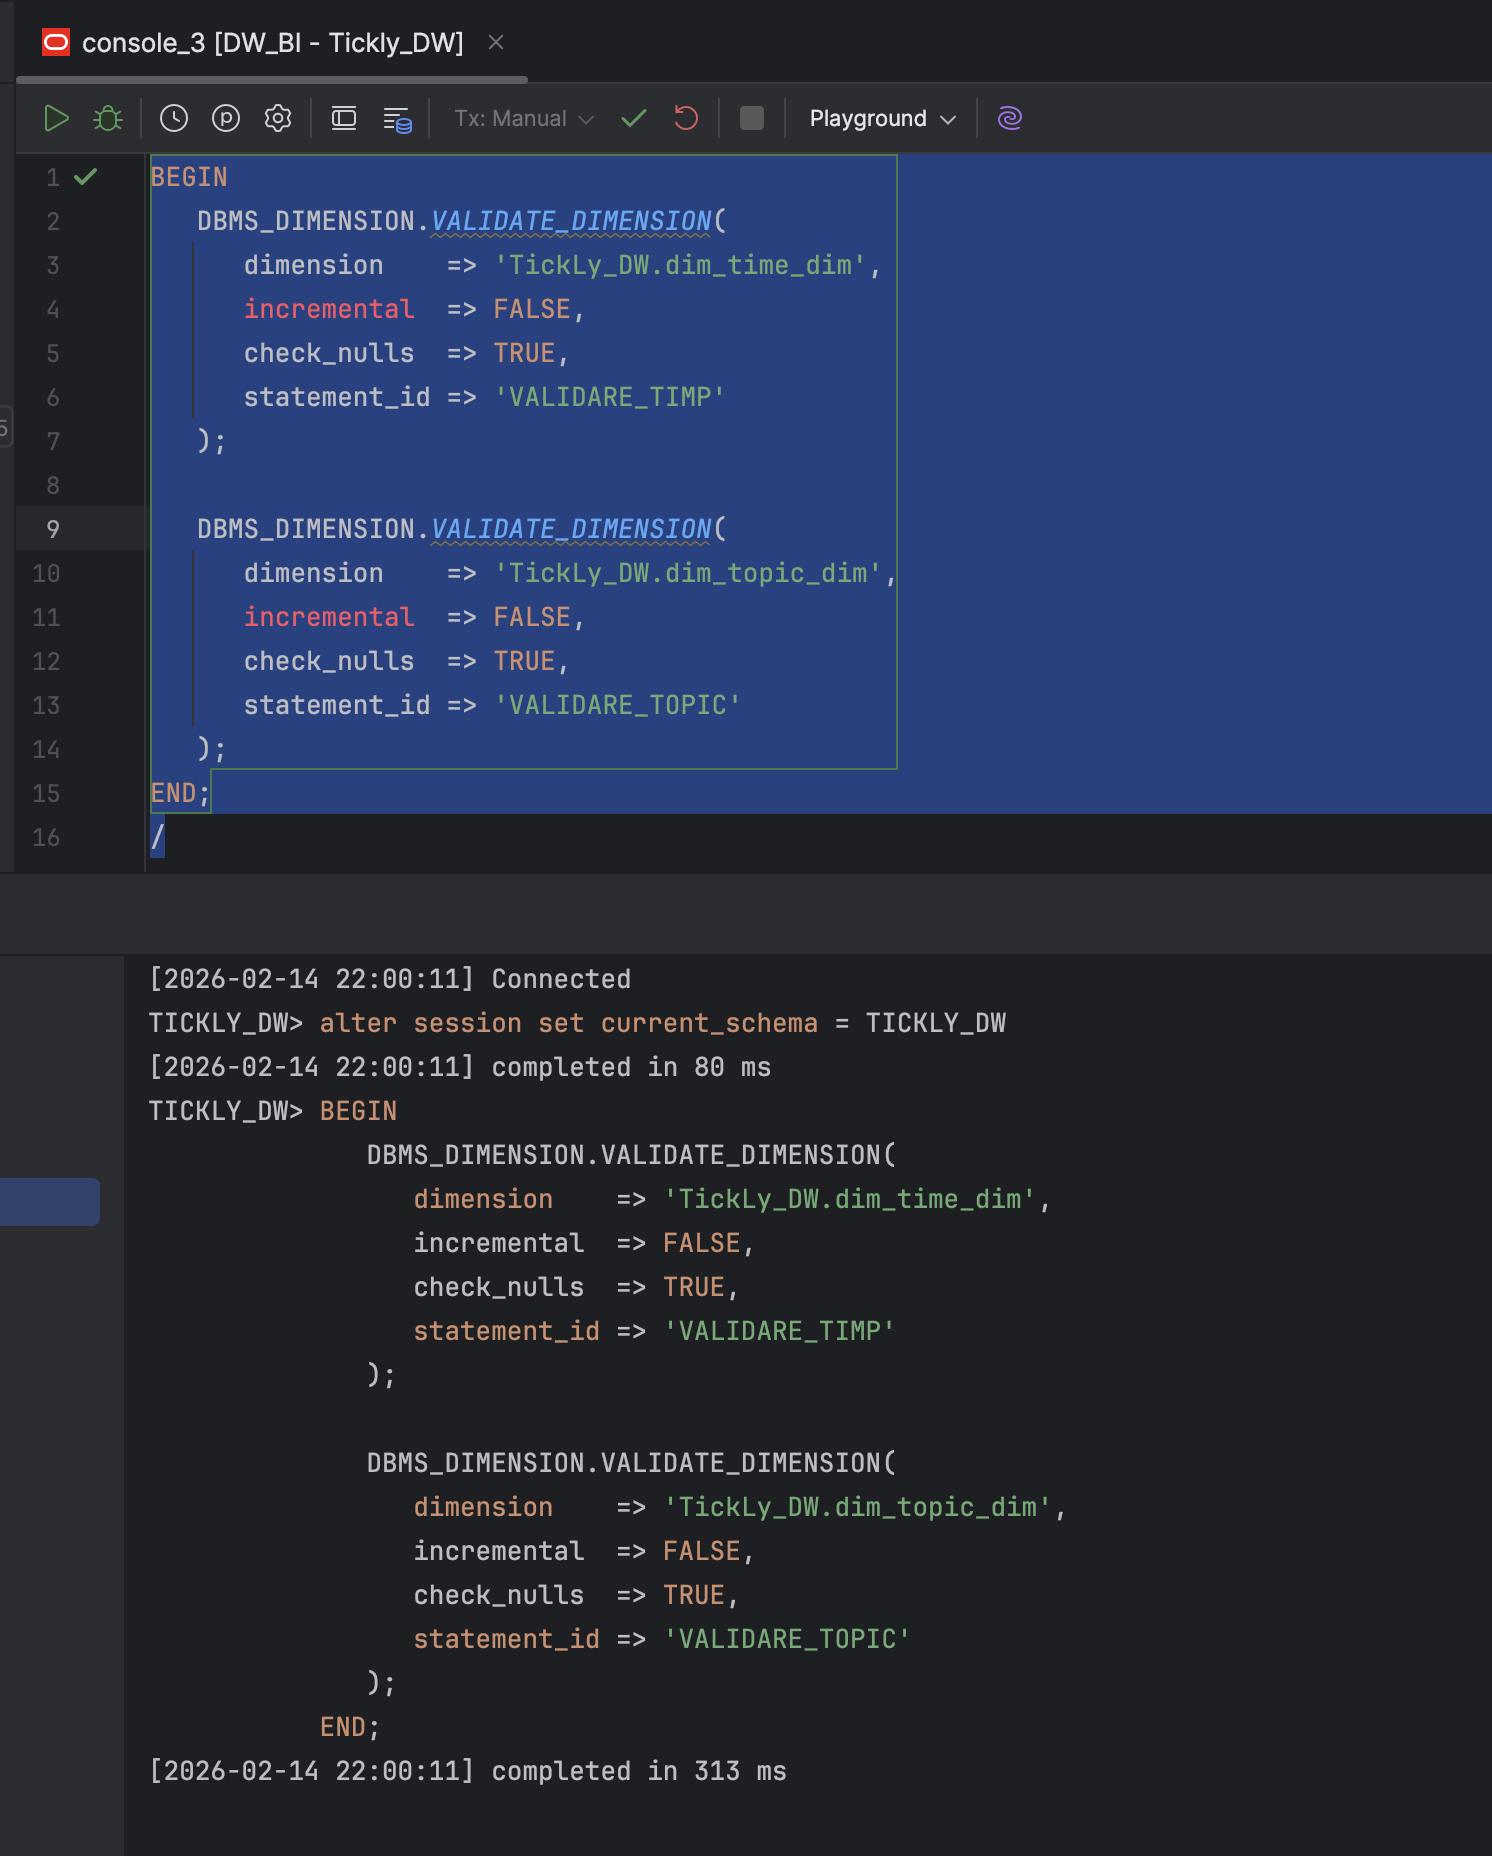
\includegraphics[width=0.6\textwidth]{../../scripts/tests/assets/validare_dimensiune.png}
    \caption{Validarea dimensiunilor}
    \label{fig:validate_dimensions}
\end{figure}

\begin{figure}[H]
    \centering
    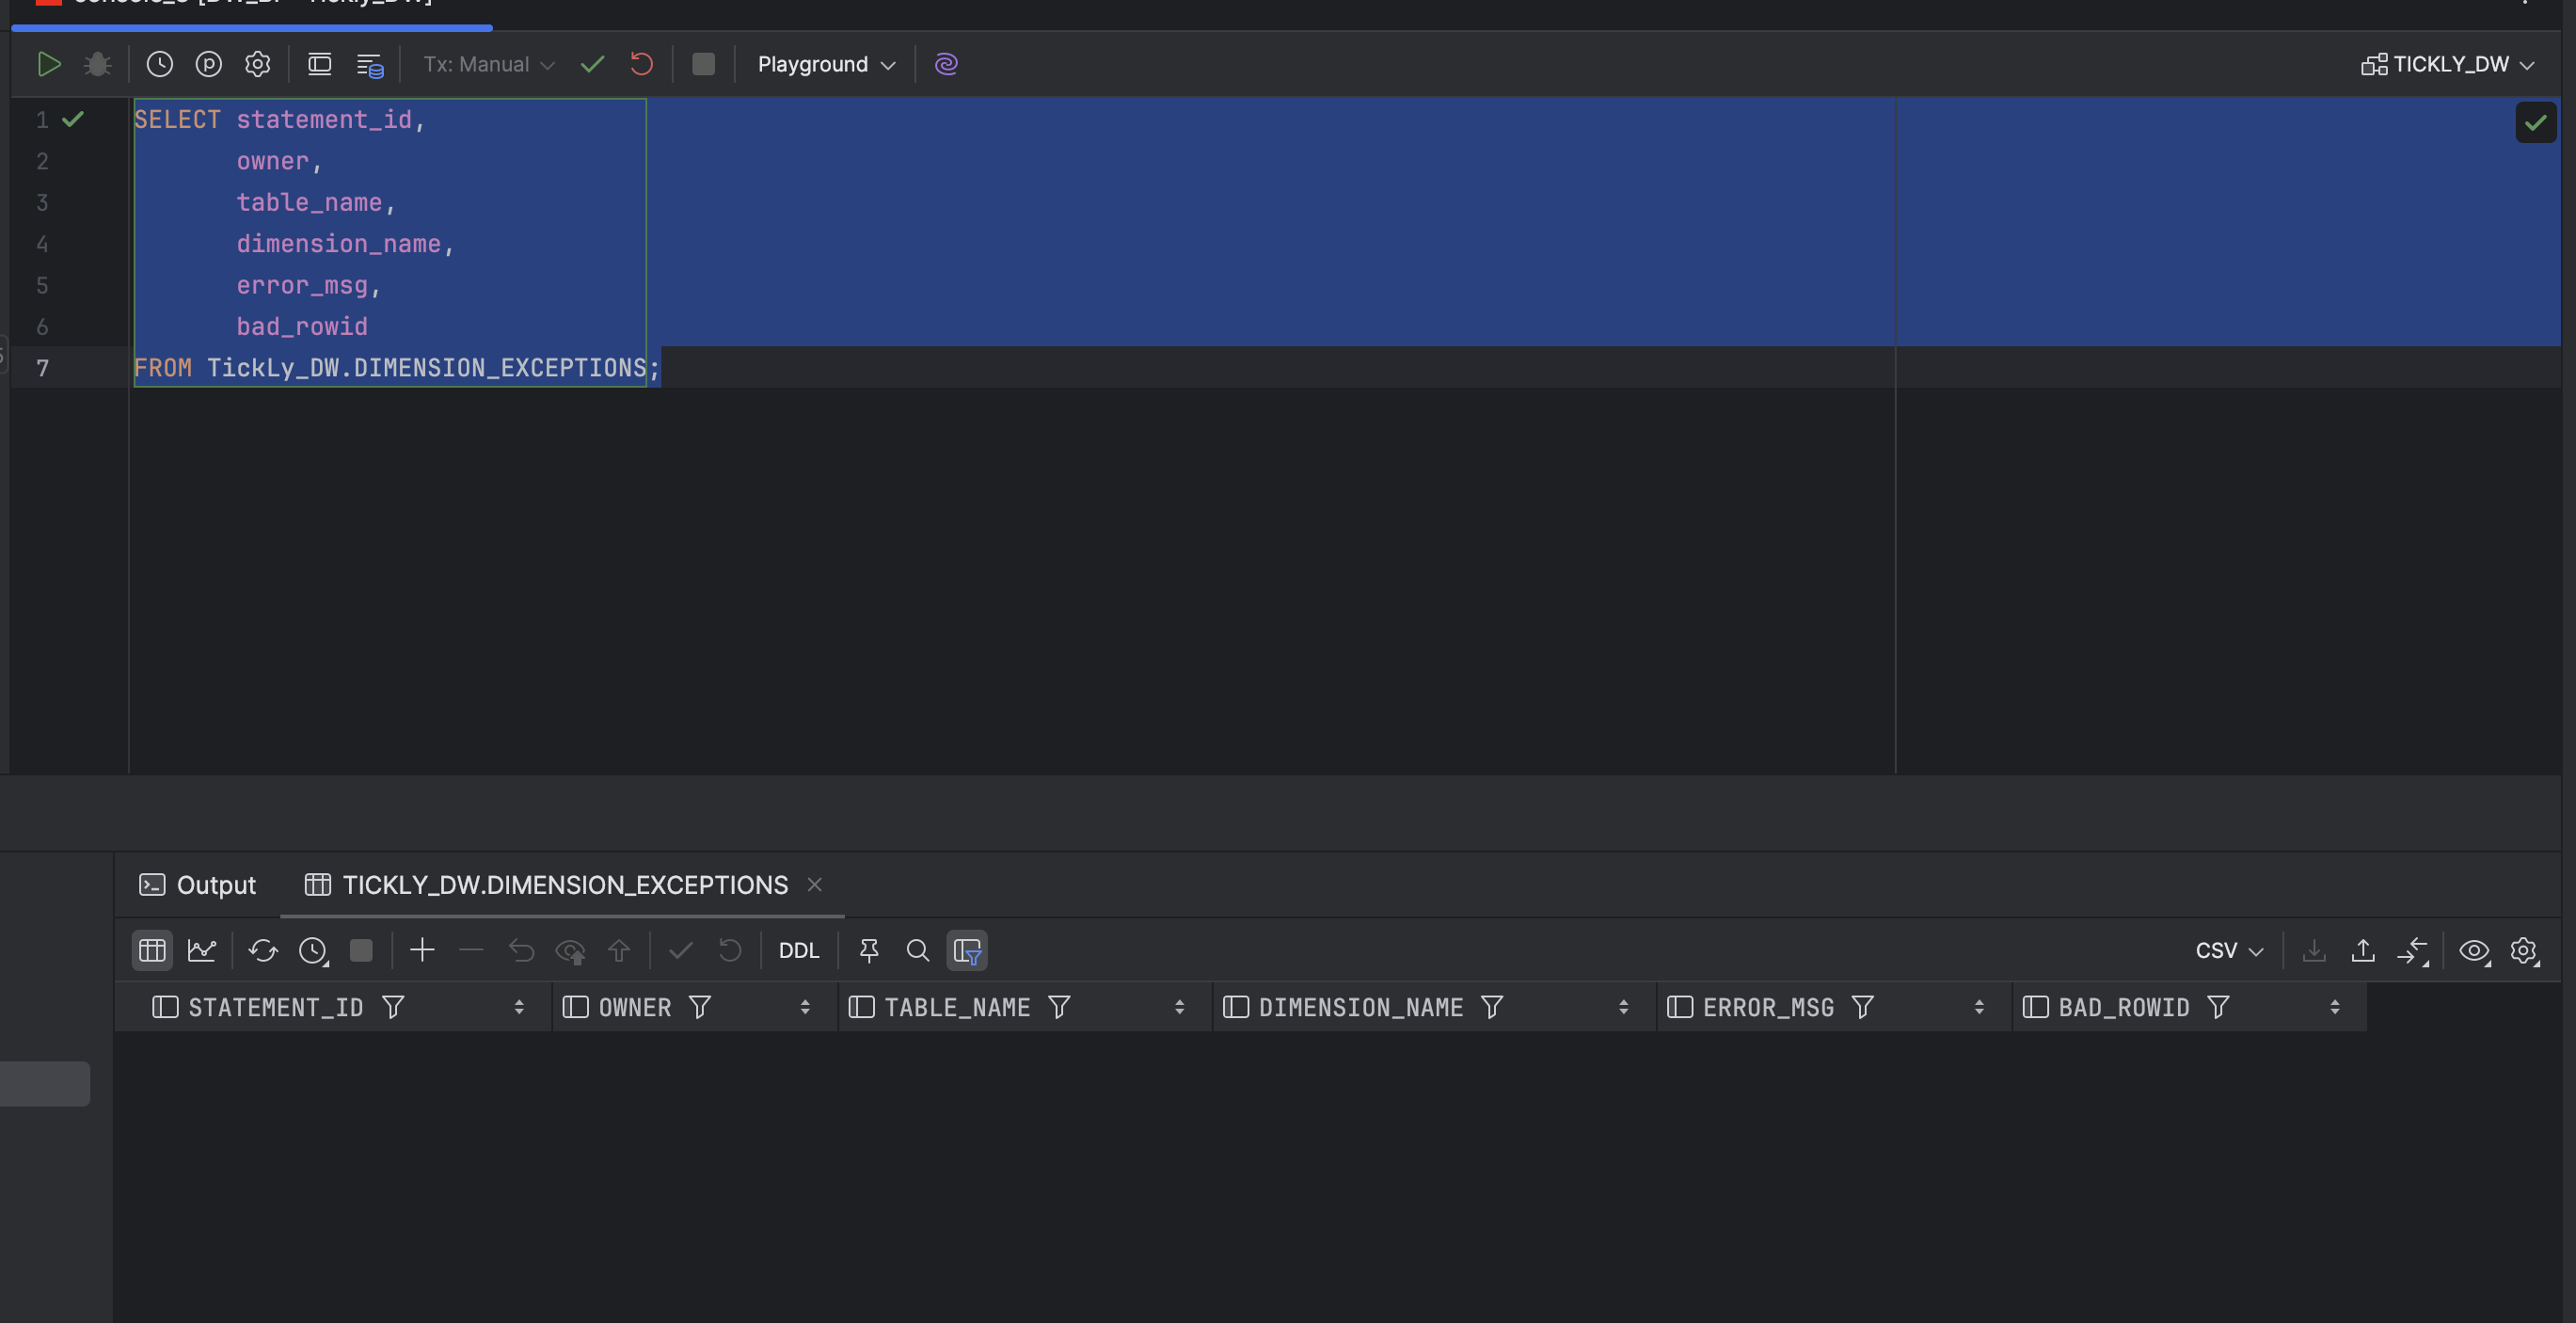
\includegraphics[width=0.6\textwidth]{../../scripts/tests/assets/verificare_validare_dimensiune.png}
    \caption{Verificarea validării dimensiunilor}
    \label{fig:verificare_validare_dimensiune}
\end{figure}

\chapter{Partiționarea Tabelelor}
\label{sec:partitii}

\section{Tabelul FACT\_TICKET — partiționare compusă}

\subsection{Tipuri de partiționare utilizate}

\begin{itemize}
    \item \textbf{Partiționare RANGE} pe \texttt{date\_creare\_key}: Datele sunt împărțite în intervale de timp ca anii. 
    \item \textbf{Subpartiționare HASH} pe \texttt{topic\_key}: Fiecare an este divizat intern în 4 subpartiții.
\end{itemize}

\subsection{Definirea partițiilor}

Partițiile RANGE sunt definite astfel:
\begin{itemize}
    \item \texttt{fact\_tickets\_2023} (VALUES LESS THAN 20240000)
    \item \texttt{fact\_tickets\_2024} (VALUES LESS THAN 20250000)
    \item \dots
    \item \texttt{fact\_tickets\_viitor} (MAXVALUE) - pentru ticketele create după anul 2030.
\end{itemize}

\section{Tabelele Dimensionale — Partiționare prin Listă}

Pentru dimensiunile \texttt{DIM\_CLIENT} și \texttt{DIM\_TOPIC}, s-a utilizat partiționarea prin liste.

\subsection{Tabelul DIM\_CLIENT}

\begin{itemize}
    \item \textbf{Partiția \texttt{p\_clienti\_fizici}}: pentru valoarea 'F'.
    \item \textbf{Partiția \texttt{p\_clienti\_juridici}}: pentru valoarea 'J'.
    \item \textbf{Partiția \texttt{p\_clienti\_altele}}: pentru valori DEFAULT.
\end{itemize}

\subsection{Tabelul DIM\_TOPIC}

Similar, dimensiunea topicurilor este partiționată pe \texttt{topic\_type} pentru a separa serviciile (manoperă, consultanță) de produsele fizice (hardware, licențe).

\begin{itemize}
    \item \textbf{Partiția \texttt{p\_topic\_servicii}}: pentru valoarea 'S'.
    \item \textbf{Partiția \texttt{p\_topic\_produse}}: pentru valoarea 'P'.
    \item \textbf{Partiția \texttt{p\_topic\_altele}}: pentru valori DEFAULT.
\end{itemize}

\section{Cereri în limbaj natural}

\textbf{1:} „Să se calculeze numărul de tichete și timpul mediu de rezolvare (în ore) pentru tichetele create în anul 2024, grupate pe departament și pe status.”

\begin{figure}[H]
    \centering
    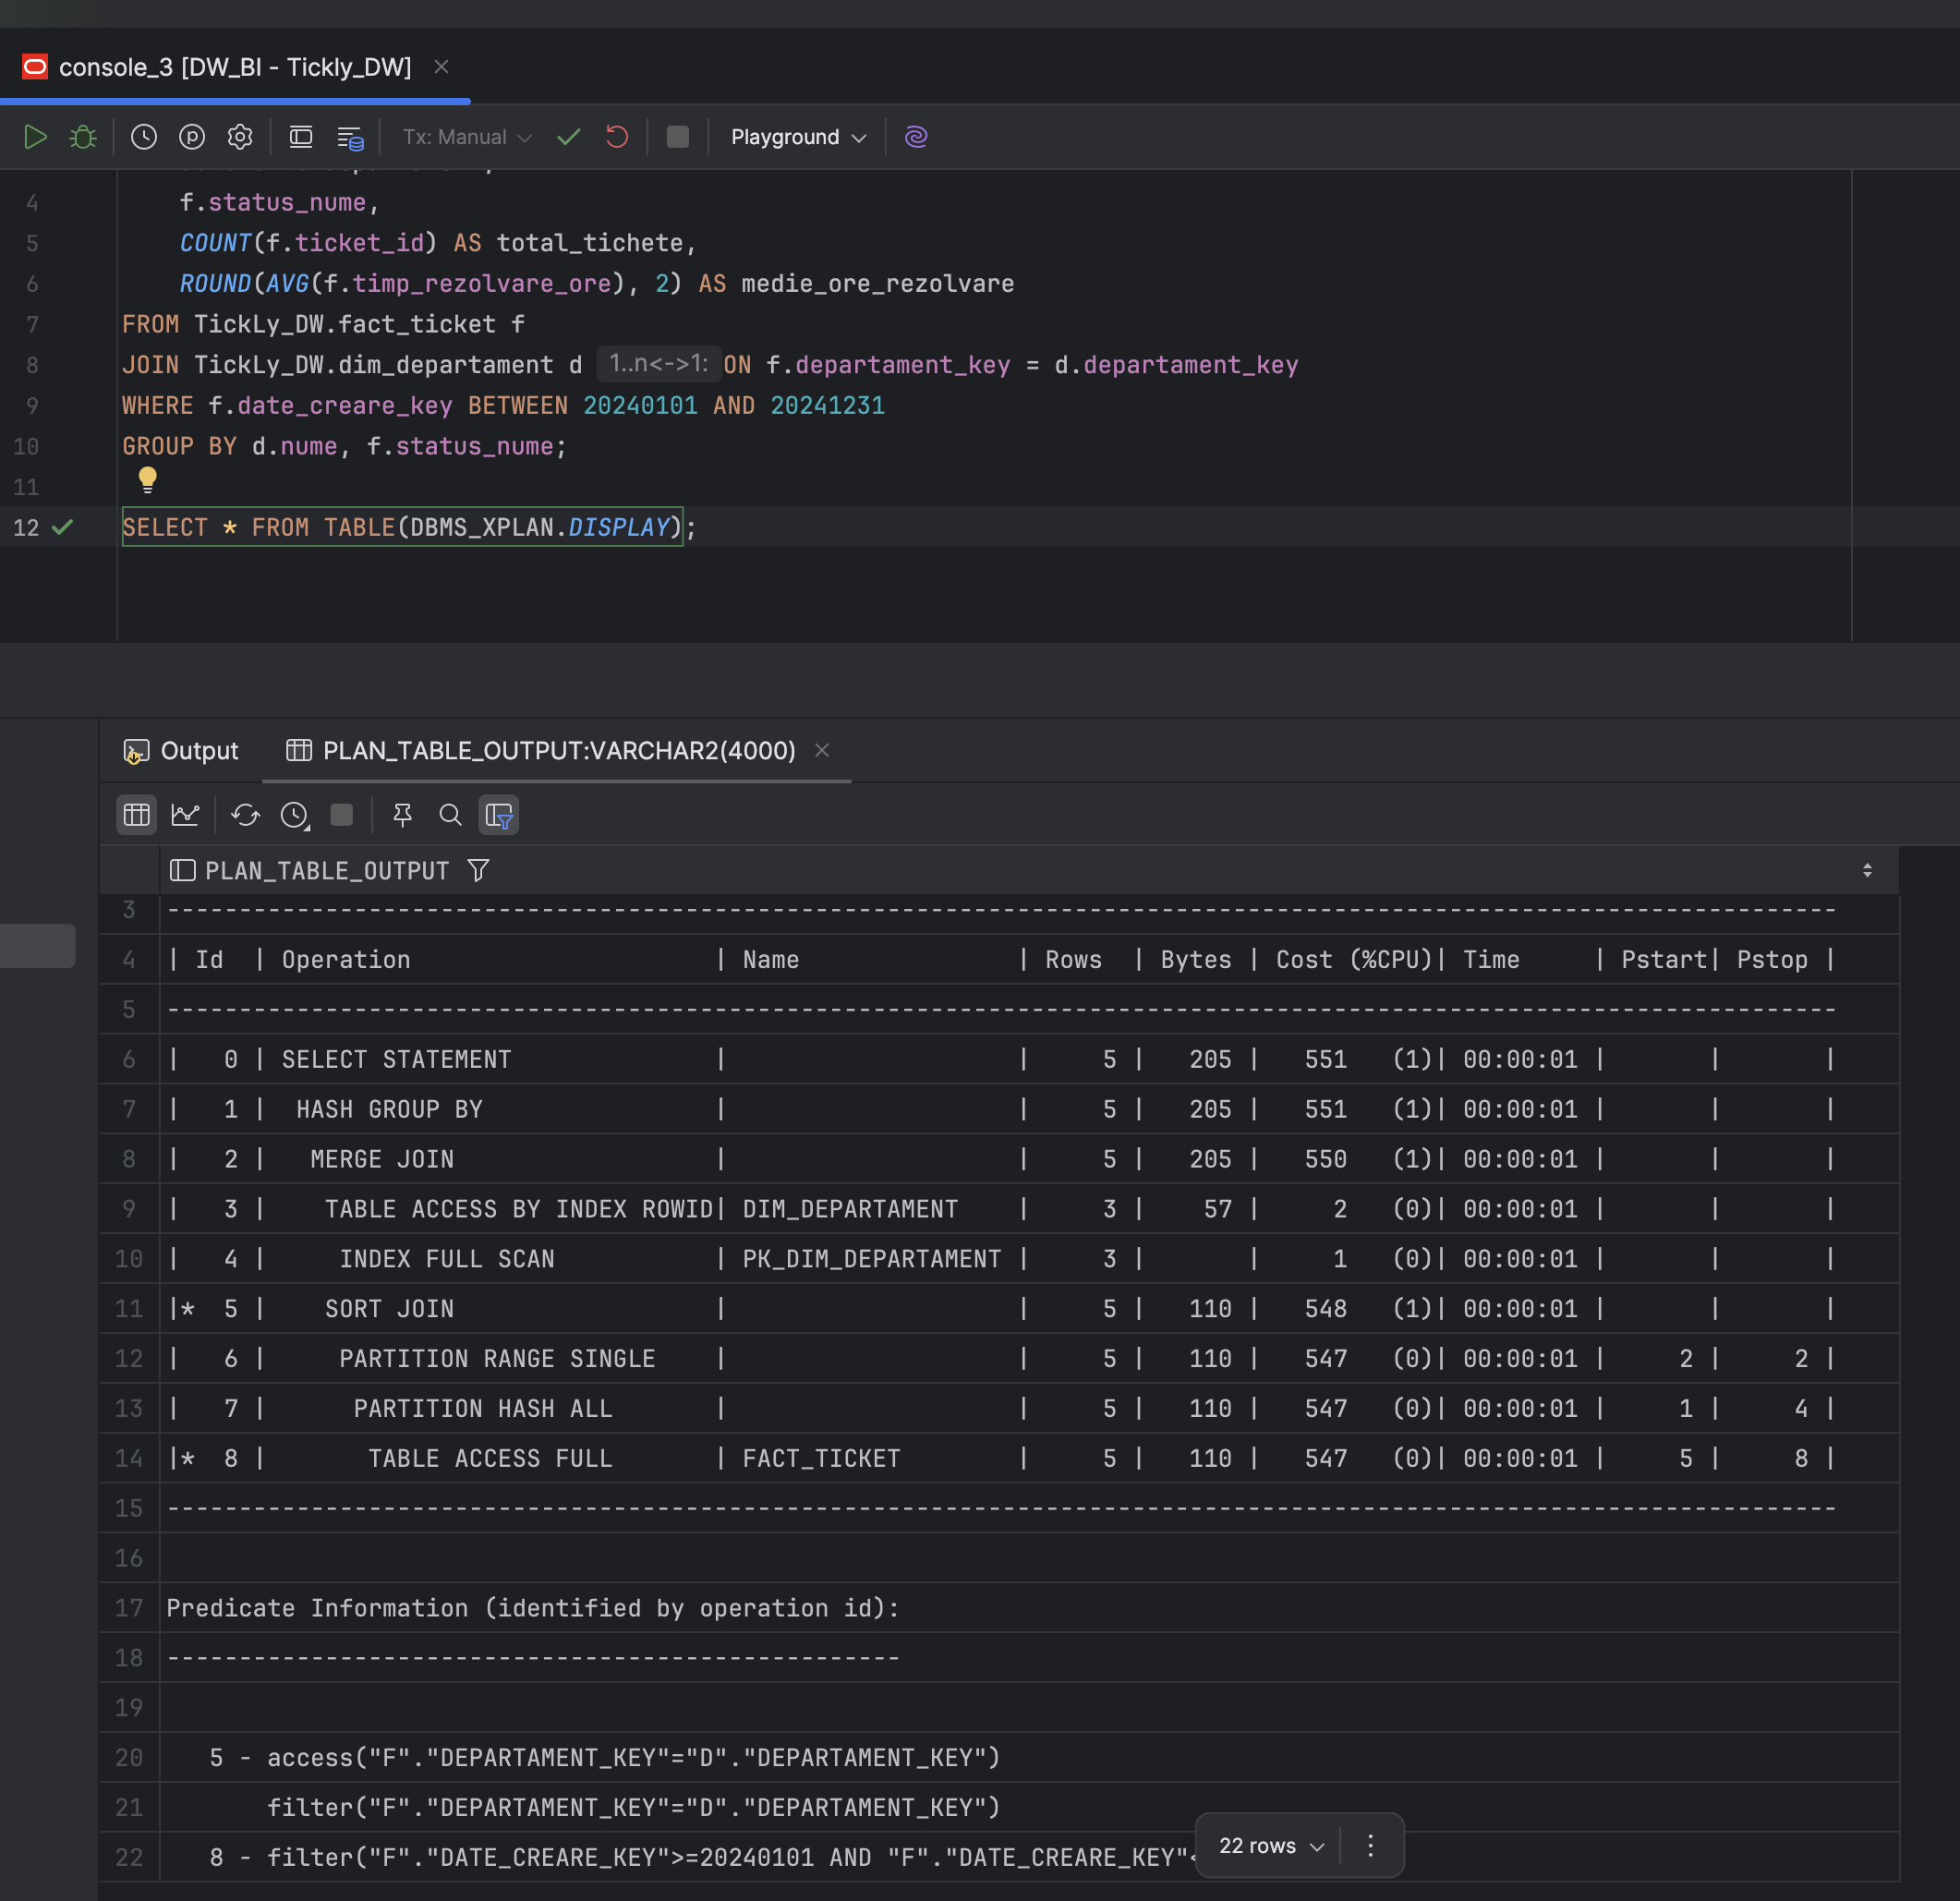
\includegraphics[width=0.6\textwidth]{../../scripts/tests/assets/partitie_range.png}
    \caption{Plan execuție: Partiționare RANGE (PARTITION RANGE SINGLE)}
    \label{fig:partitie_range}
\end{figure}

\textbf{2:} „Analiza performanței pentru un anumit Topic critic (ex: ID 105) în anul 2024.”

\begin{figure}[H]
    \centering
    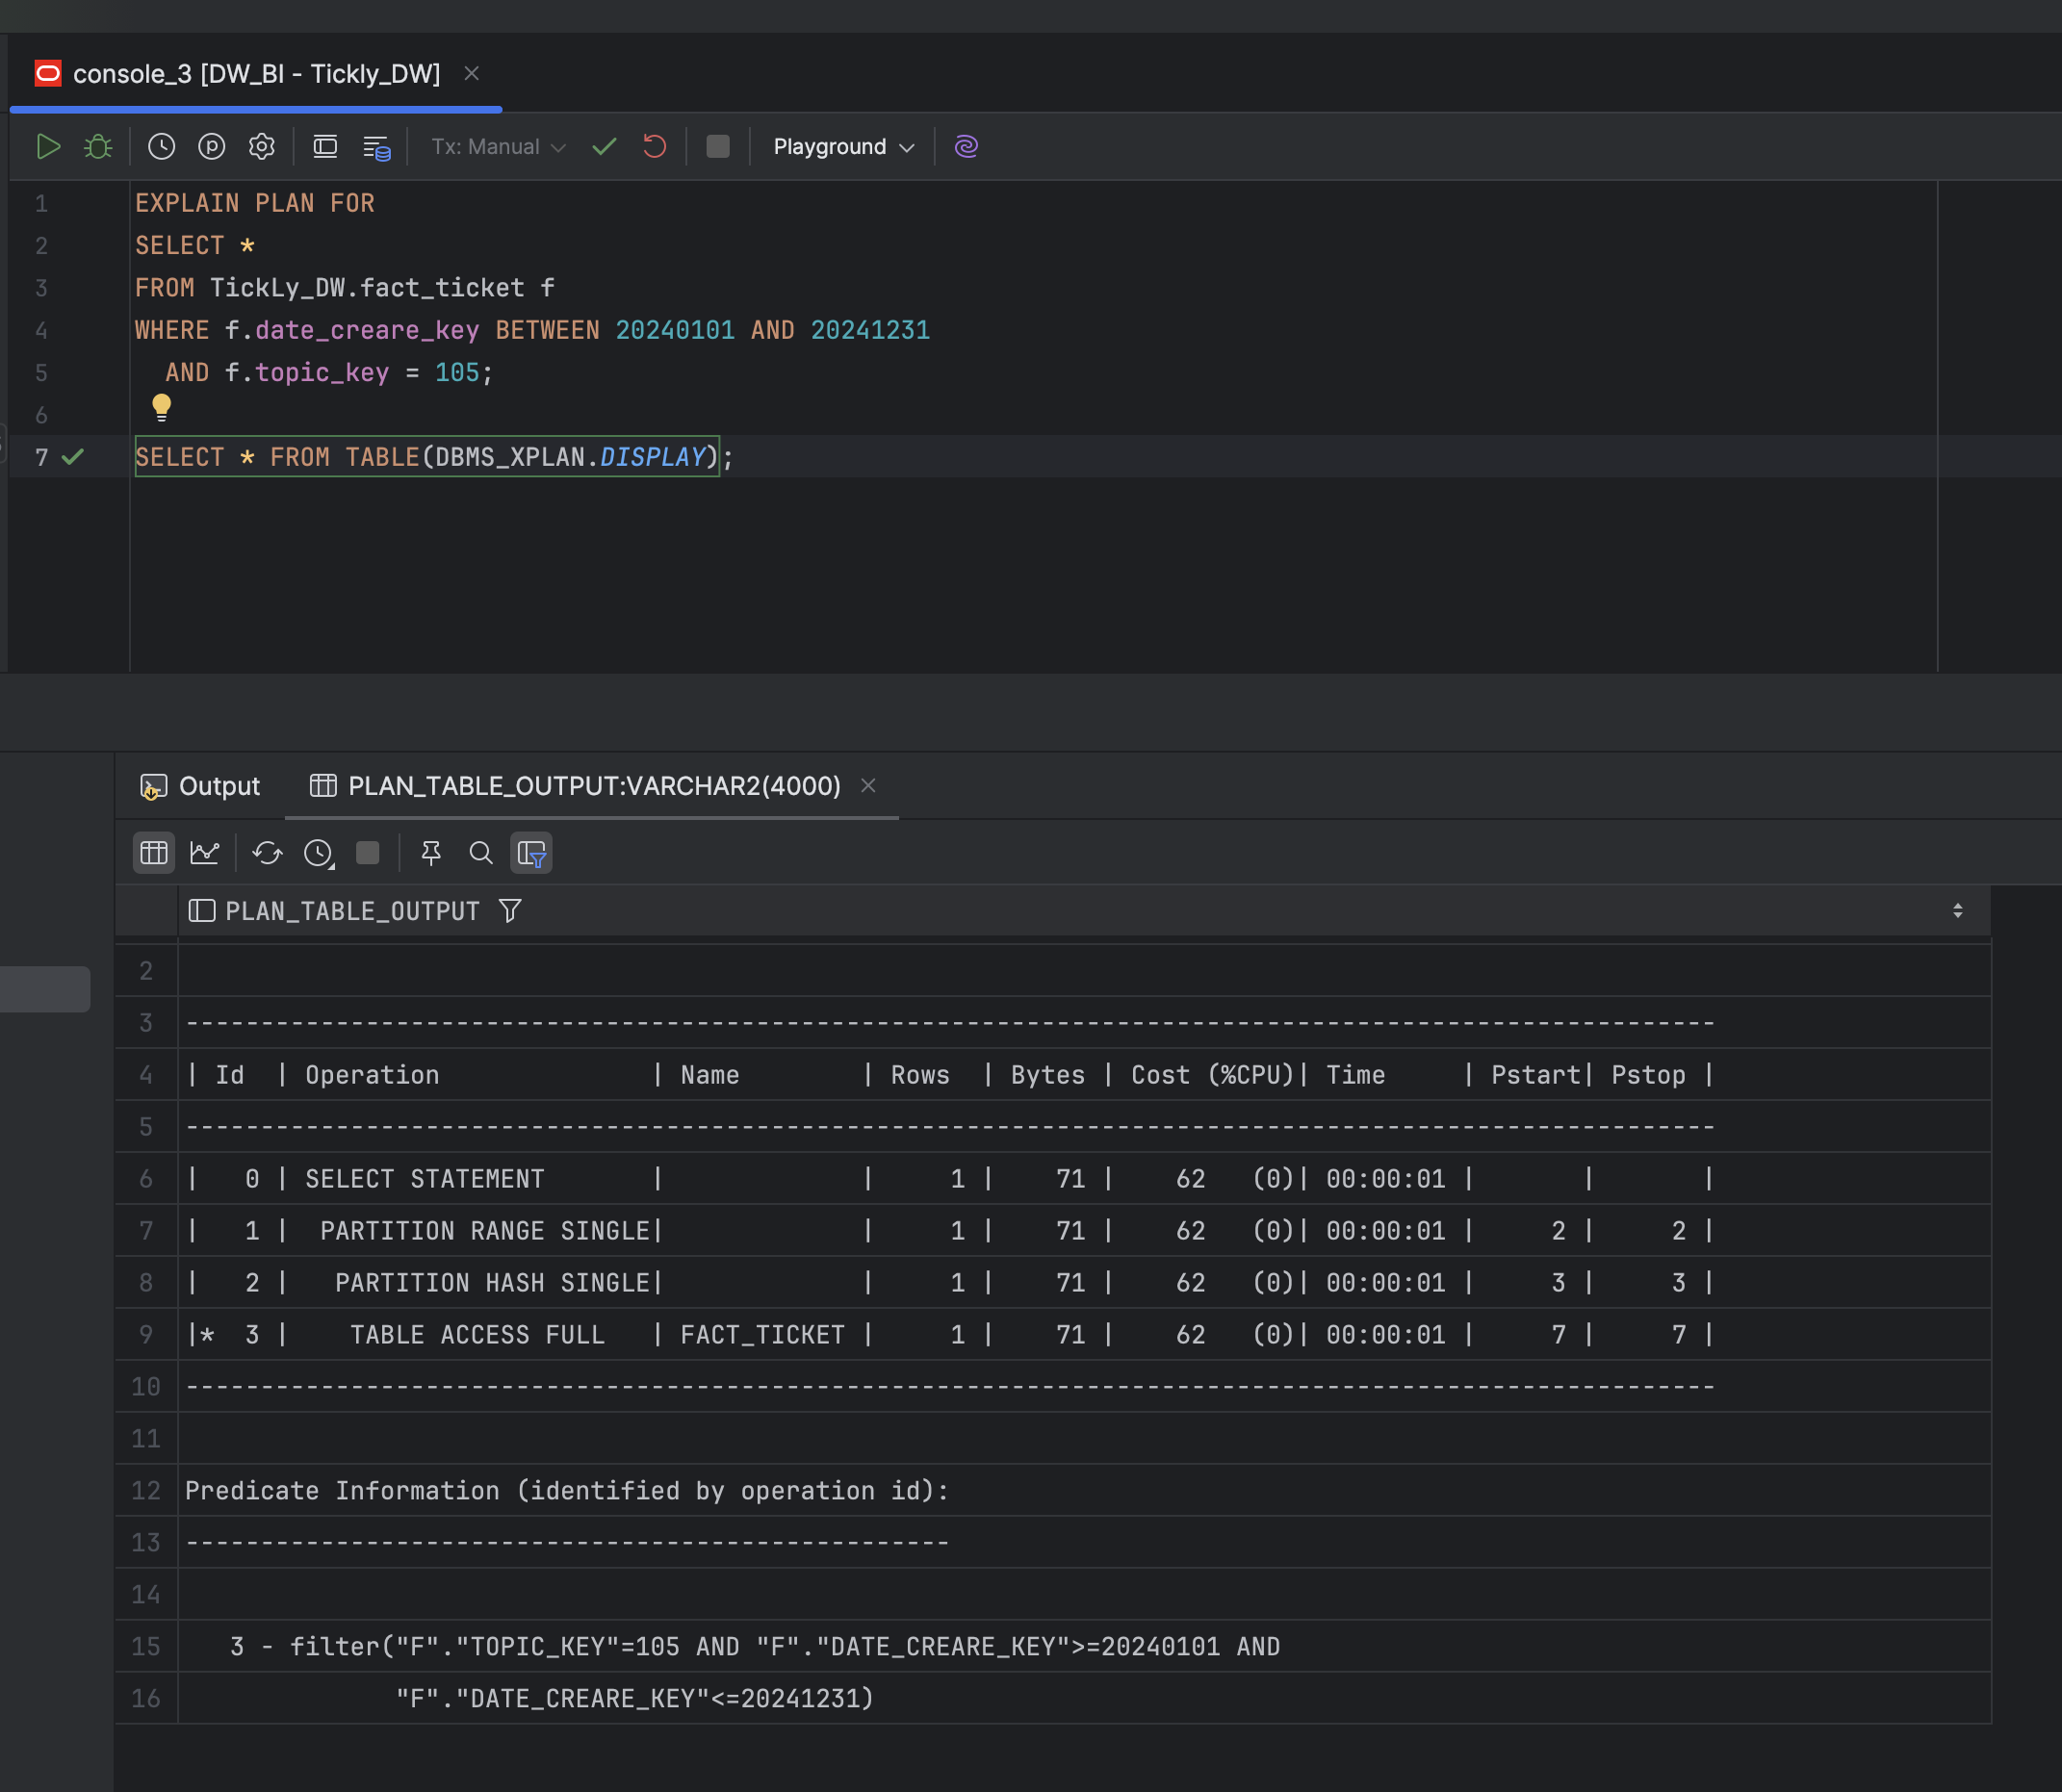
\includegraphics[width=0.6\textwidth]{../../scripts/tests/assets/partitie_range_hash.png}
    \caption{Plan execuție: Partiționare RANGE și HASH}
    \label{fig:partitie_range_hash}
\end{figure}

\textbf{3:} „Lista tuturor clienților persoane juridice și CUI-ul acestora.”

\begin{figure}[H]
    \centering
    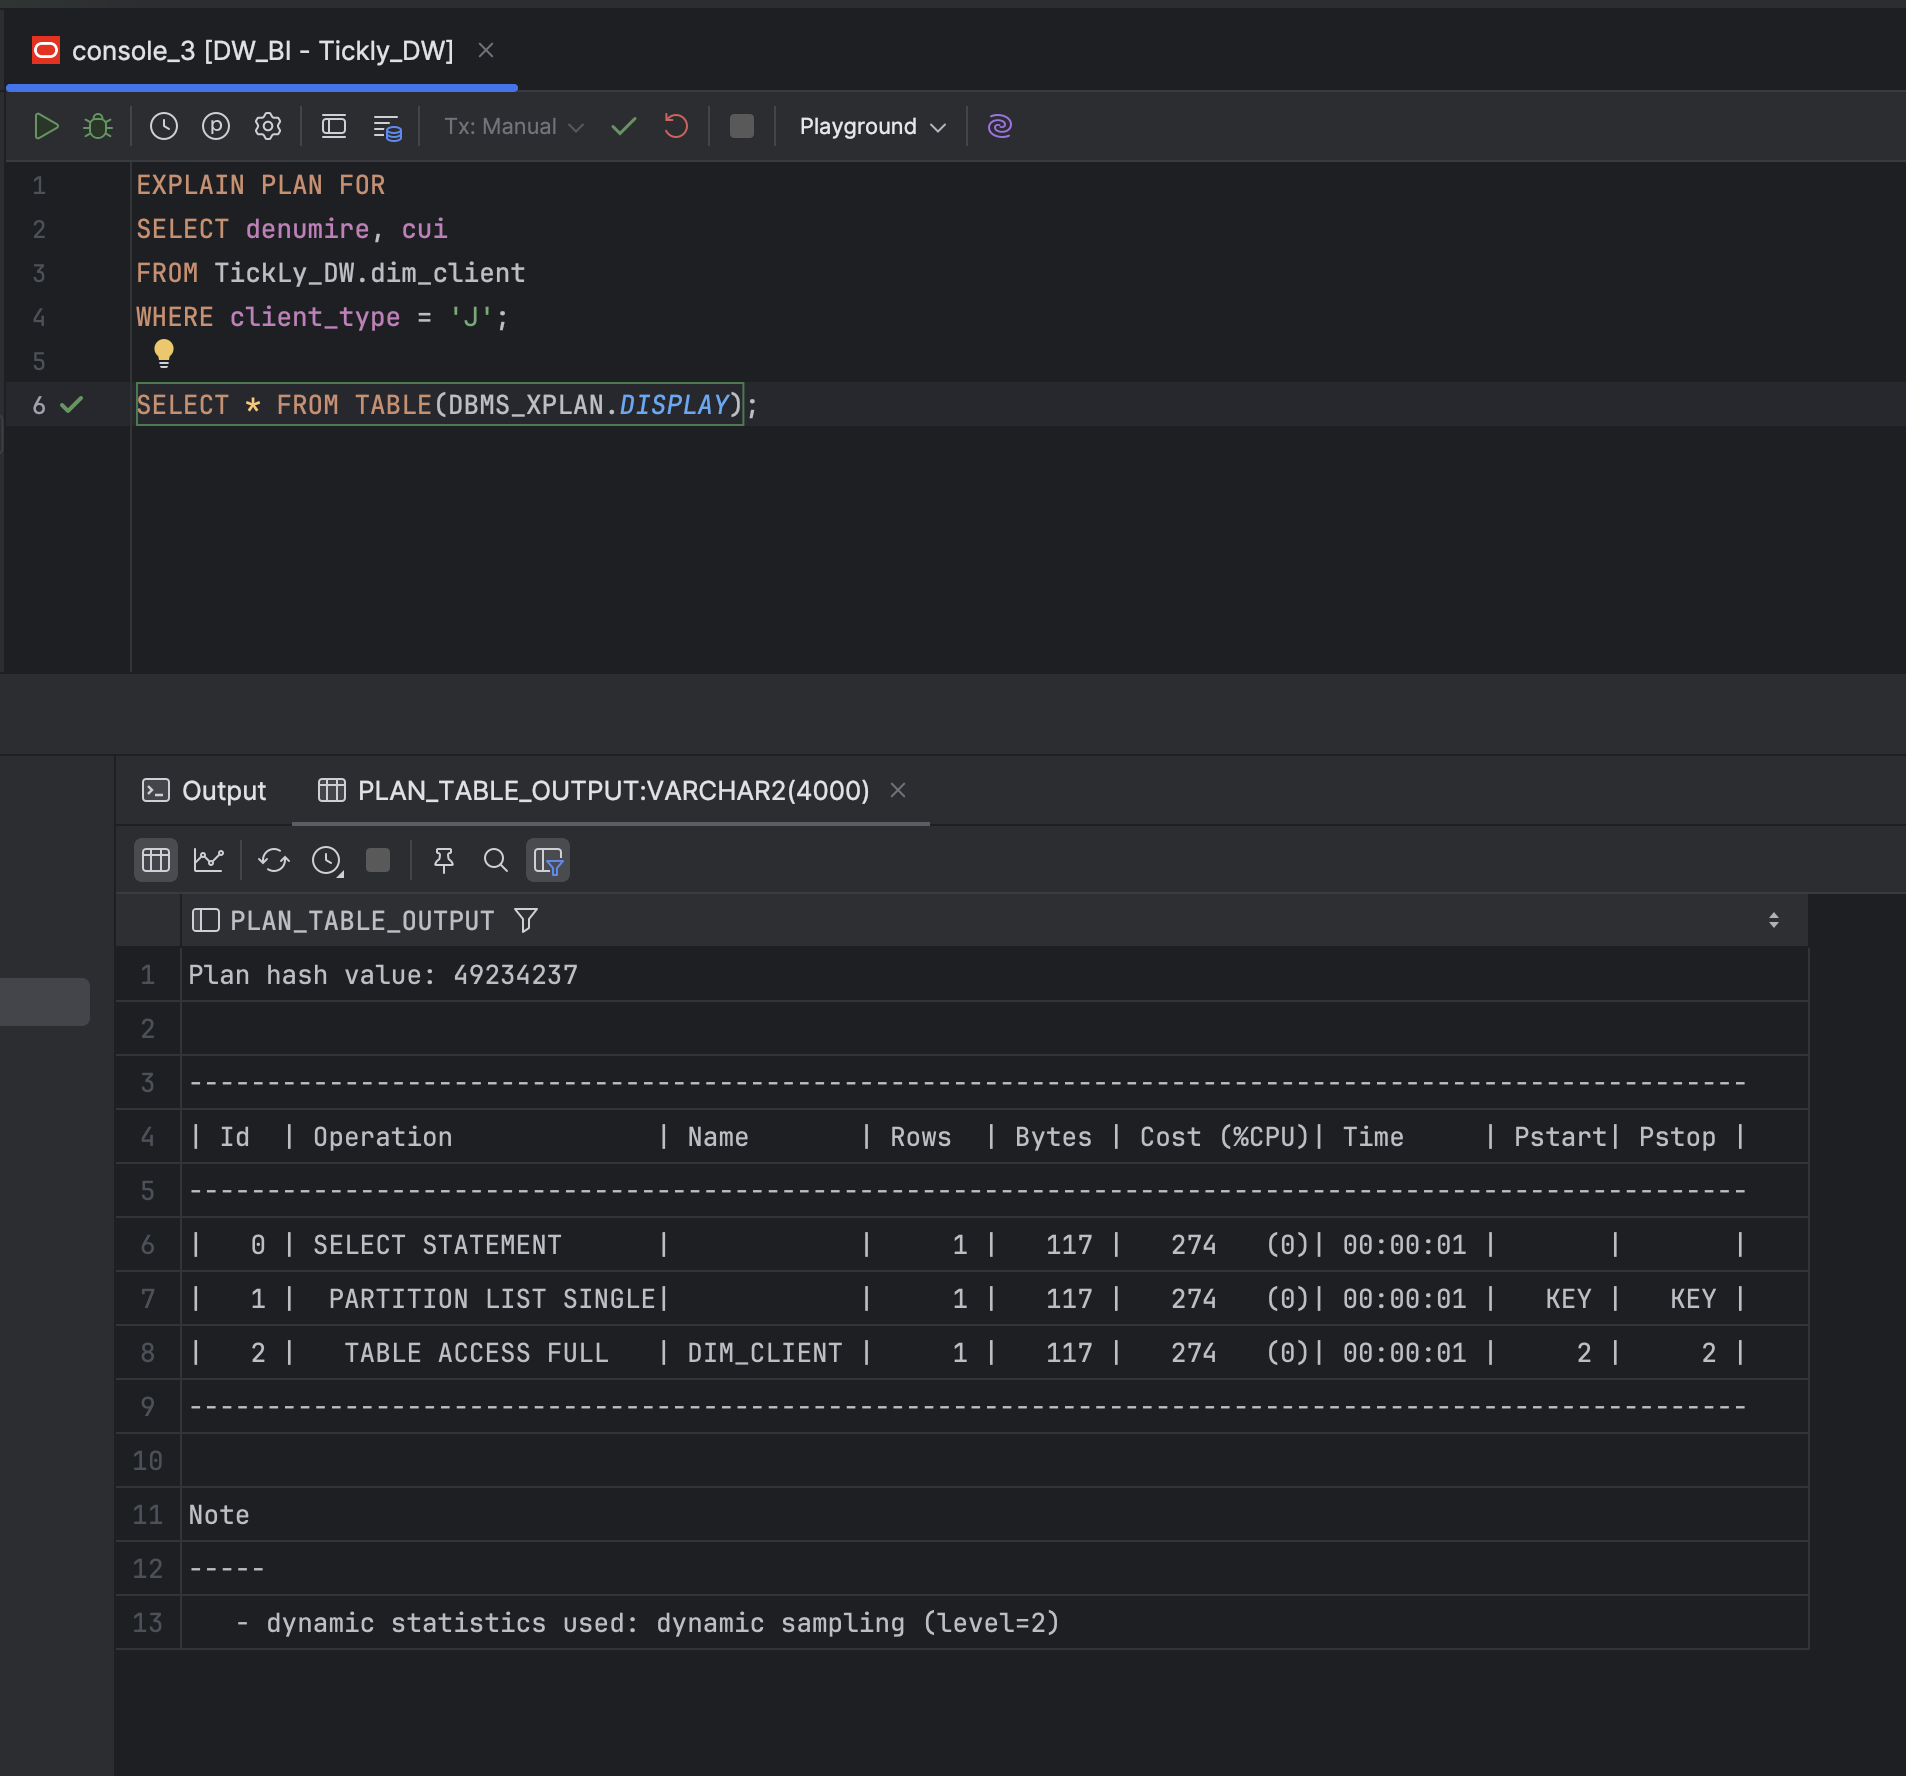
\includegraphics[width=0.6\textwidth]{../../scripts/tests/assets/partitie_list.png} 
    \caption{Plan execuție: Partiționare LIST pe DIM\_CLIENT}
    \label{fig:partitie_list_client}
\end{figure}

\chapter{Indecșii Specifici OLTP și Depozit}
\label{sec:indecsi}

\section{Indecși OLTP (schema TickLy)}

\subsubsection{Pe tabelul TICKET și tabele copil}

\begin{itemize}
    \item \textbf{idx\_ticket\_client}, \textbf{idx\_ticket\_dept}, \textbf{idx\_ticket\_status}, \textbf{idx\_ticket\_prioritate}, \textbf{idx\_ticket\_categ}: B-tree pe coloanele FK, pentru join-uri și filtre
    \item \textbf{idx\_ticket\_data\_creare}: B-tree pe \texttt{data\_creare} — pentru filtre și sortări temporale
    \item \textbf{idx\_comm\_client\_tid}, \textbf{idx\_comm\_agent\_tid}: pe \texttt{comment\_client(ticket\_id)}, \texttt{comment\_agent(ticket\_id)} — listare comentarii per ticket
    \item \textbf{idx\_hist\_ticket\_tid}: pe \texttt{ticket\_history(ticket\_id)} — istoric evenimente per ticket
    \item \textbf{idx\_atasament\_ticket\_id}: pe \texttt{atasament(ticket\_id)}
    \item \textbf{idx\_ticket\_agent\_rev}: pe \texttt{ticket\_agent(agent\_id)} — tichete per agent
    \item \textbf{idx\_ticket\_tag\_rev}: pe \texttt{ticket\_tag(tag\_id)} — tichete per tag
\end{itemize}

\subsubsection{Indecși function-based (căutări case-insensitive)}

\begin{itemize}
    \item \textbf{idx\_client\_nume\_upper}, \textbf{idx\_client\_prenume\_upper}: pe \texttt{UPPER(nume)}, \texttt{UPPER(prenume)} în \texttt{client\_fizica}
    \item \textbf{idx\_juridic\_denumire\_upper}: pe \texttt{UPPER(denumire)} în \texttt{client\_juridica}
\end{itemize}

\section{Indecși OLAP (schema TickLy\_DW)}

\subsubsection{Pe tabelul de fapte și bridge}

\begin{itemize}
    \item \textbf{bidx\_fact\_status}: bitmap pe \texttt{fact\_ticket(status\_id)} — cardinalitate mică
    \item \textbf{bidx\_fact\_prioritate}: bitmap pe \texttt{fact\_ticket(prioritate\_id)}
    \item \textbf{bidx\_bridge\_tag}: bitmap pe \texttt{bridge\_ticket\_tag(tag\_key)}
    \item \textbf{idx\_bridge\_ticket\_id}: B-tree pe \texttt{bridge\_ticket\_tag(fact\_ticket\_id)} — cardinalitate mare
\end{itemize}

\subsubsection{Pe dimensiuni}

\begin{itemize}
    \item \textbf{idx\_dim\_client\_cnp}: B-tree pe \texttt{dim\_client(cnp)} — lookup și căutări pe CNP
\end{itemize}

\section{Cereri SQL și Plan de Execuție}

\begin{enumerate}
    \item \textbf{OLTP — index function-based pe \texttt{client\_fizica}}
    \begin{itemize}
        \item \textbf{1:} „Să se afișeze datele (identificator, CNP, nume, prenume) persoanelor fizice care au numele egal cu «RADU»”
    \end{itemize}

    \begin{figure}[H]
        \centering
        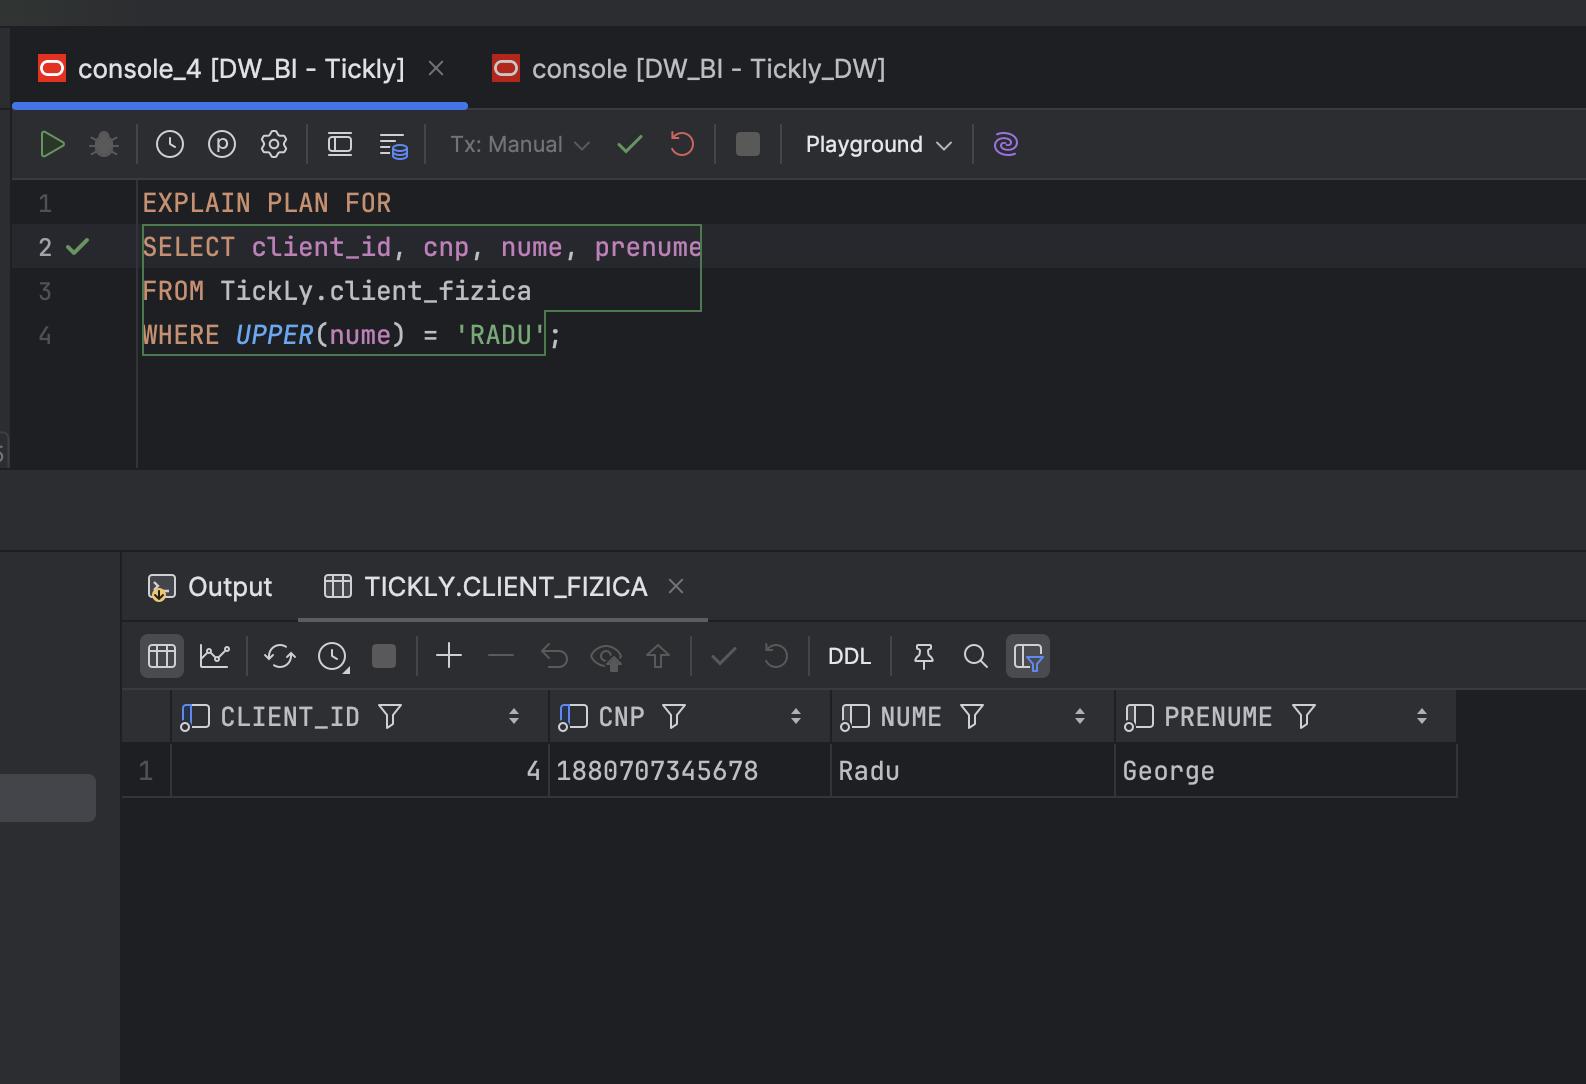
\includegraphics[width=0.6\textwidth]{./assets/indexes/test_1.png}
        \caption{Rulare query 1}
        \label{fig:rulare_query_1}
    \end{figure}

    \begin{figure}[H]
        \centering
        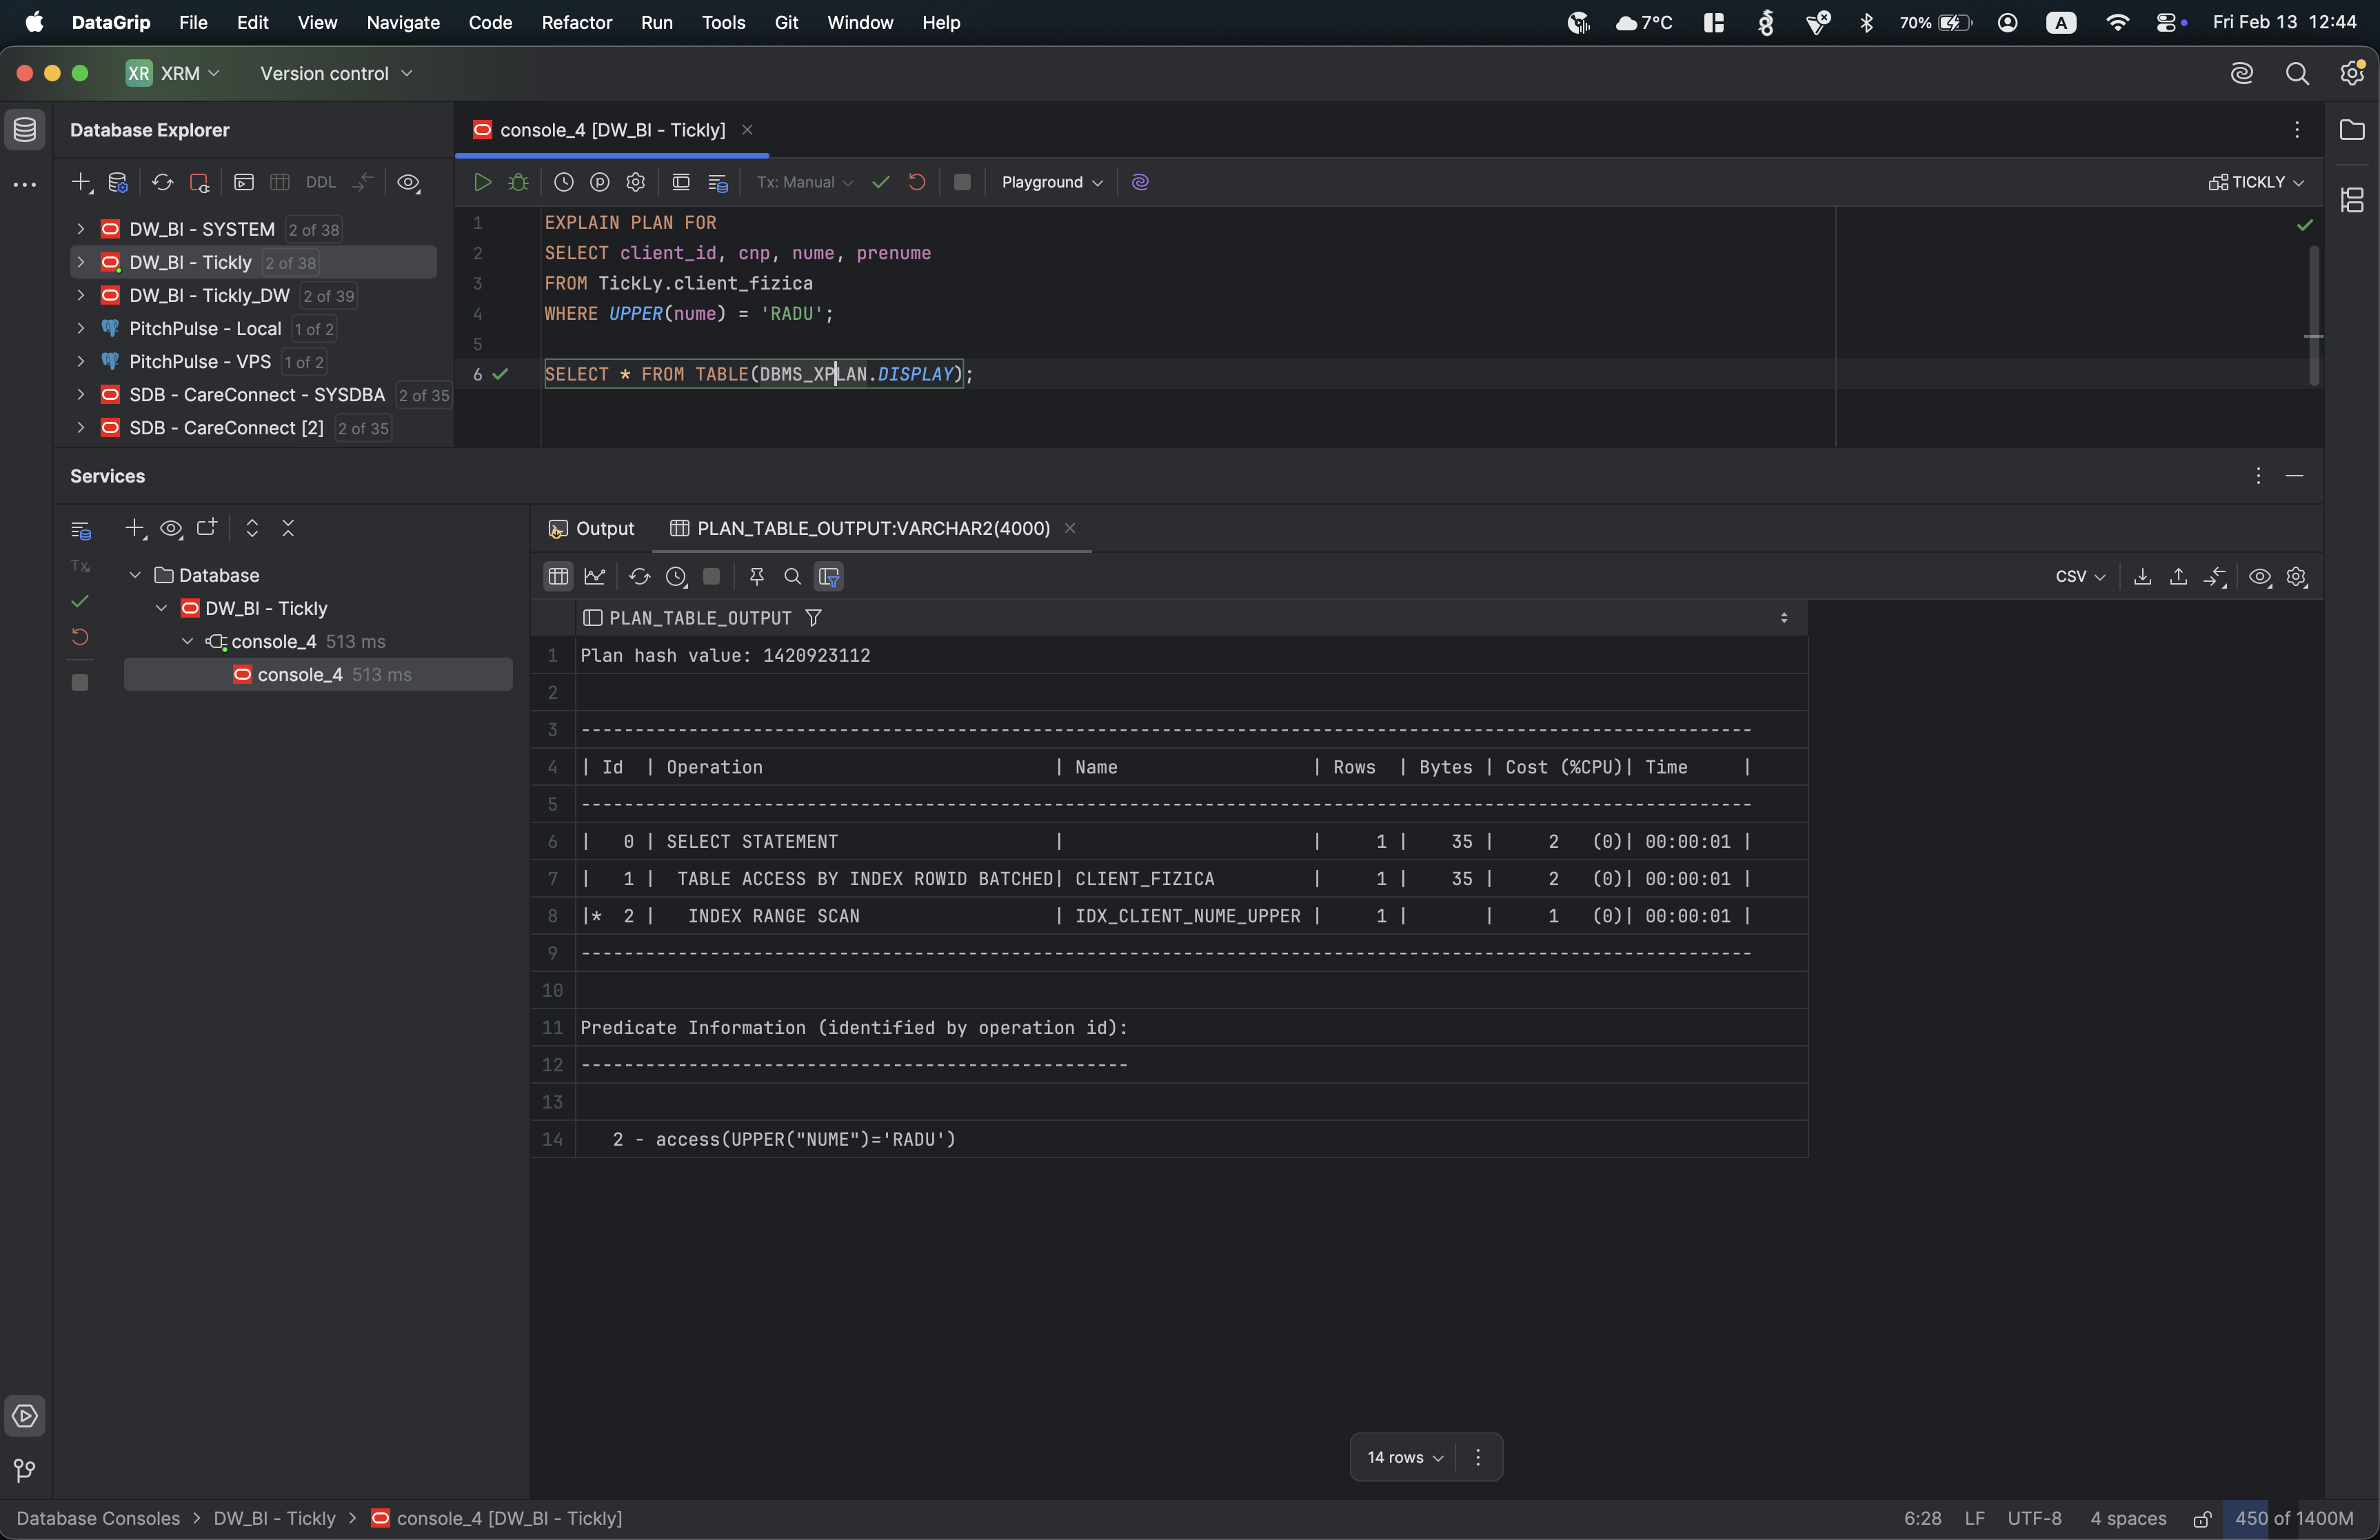
\includegraphics[width=0.6\textwidth]{../../scripts/tests/assets/oltp_client_index_explain.png}
        \caption{Plan de execuție query 1}
        \label{fig:plan_executie_query_1}
    \end{figure}

    \item \textbf{OLTP — index pe \texttt{ticket.data\_creare}}
    \begin{itemize}
        \item \textbf{2:} „Să se afișeze identificatorul, titlul, statusul și data creării pentru toate tichetele create în anul 2024, între luna februarie și luna decembrie.”
    \end{itemize}

    \begin{figure}[H]
        \centering
        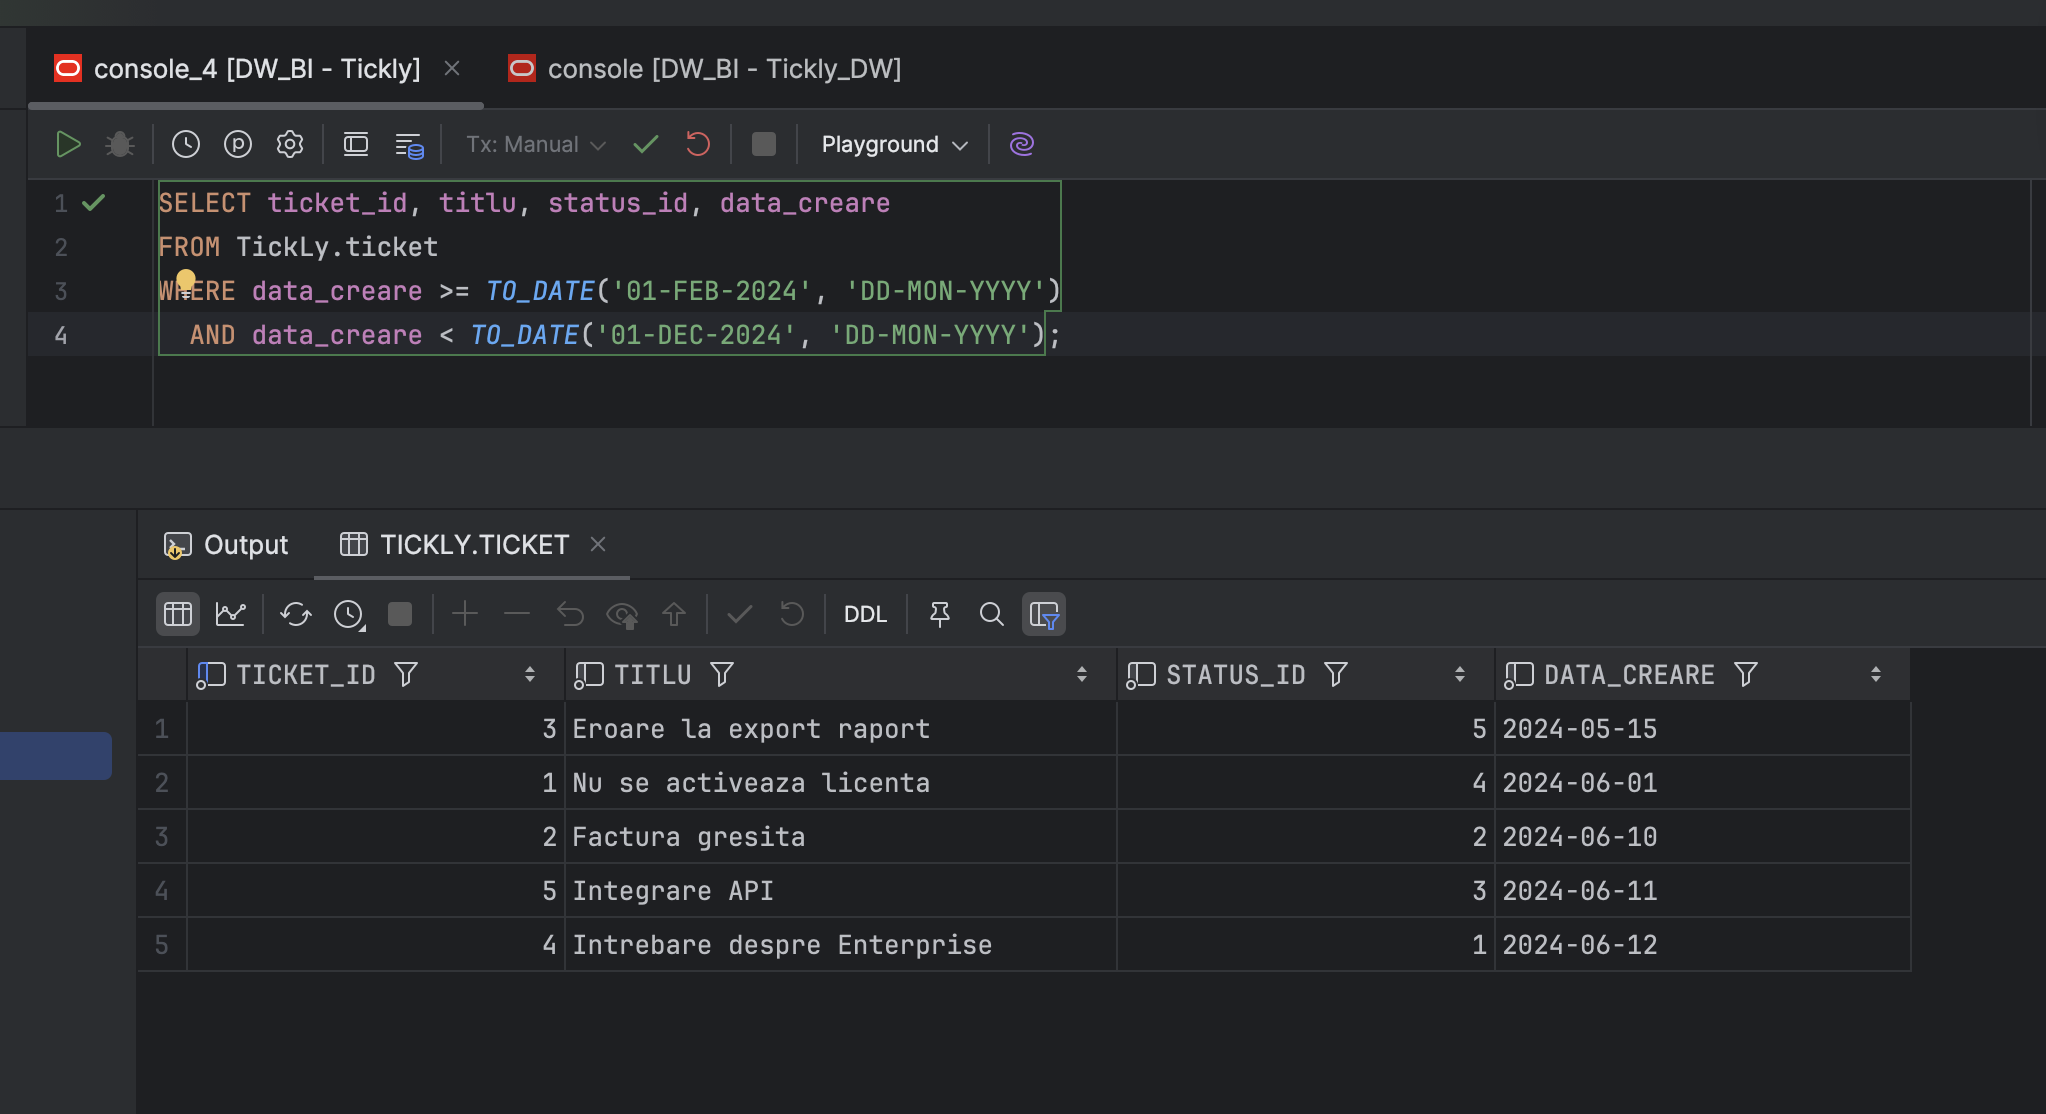
\includegraphics[width=0.6\textwidth]{./assets/indexes/test_2.png}
        \caption{Rulare query 2}
        \label{fig:rulare_query_2}
    \end{figure}

    \begin{figure}[H]
        \centering
        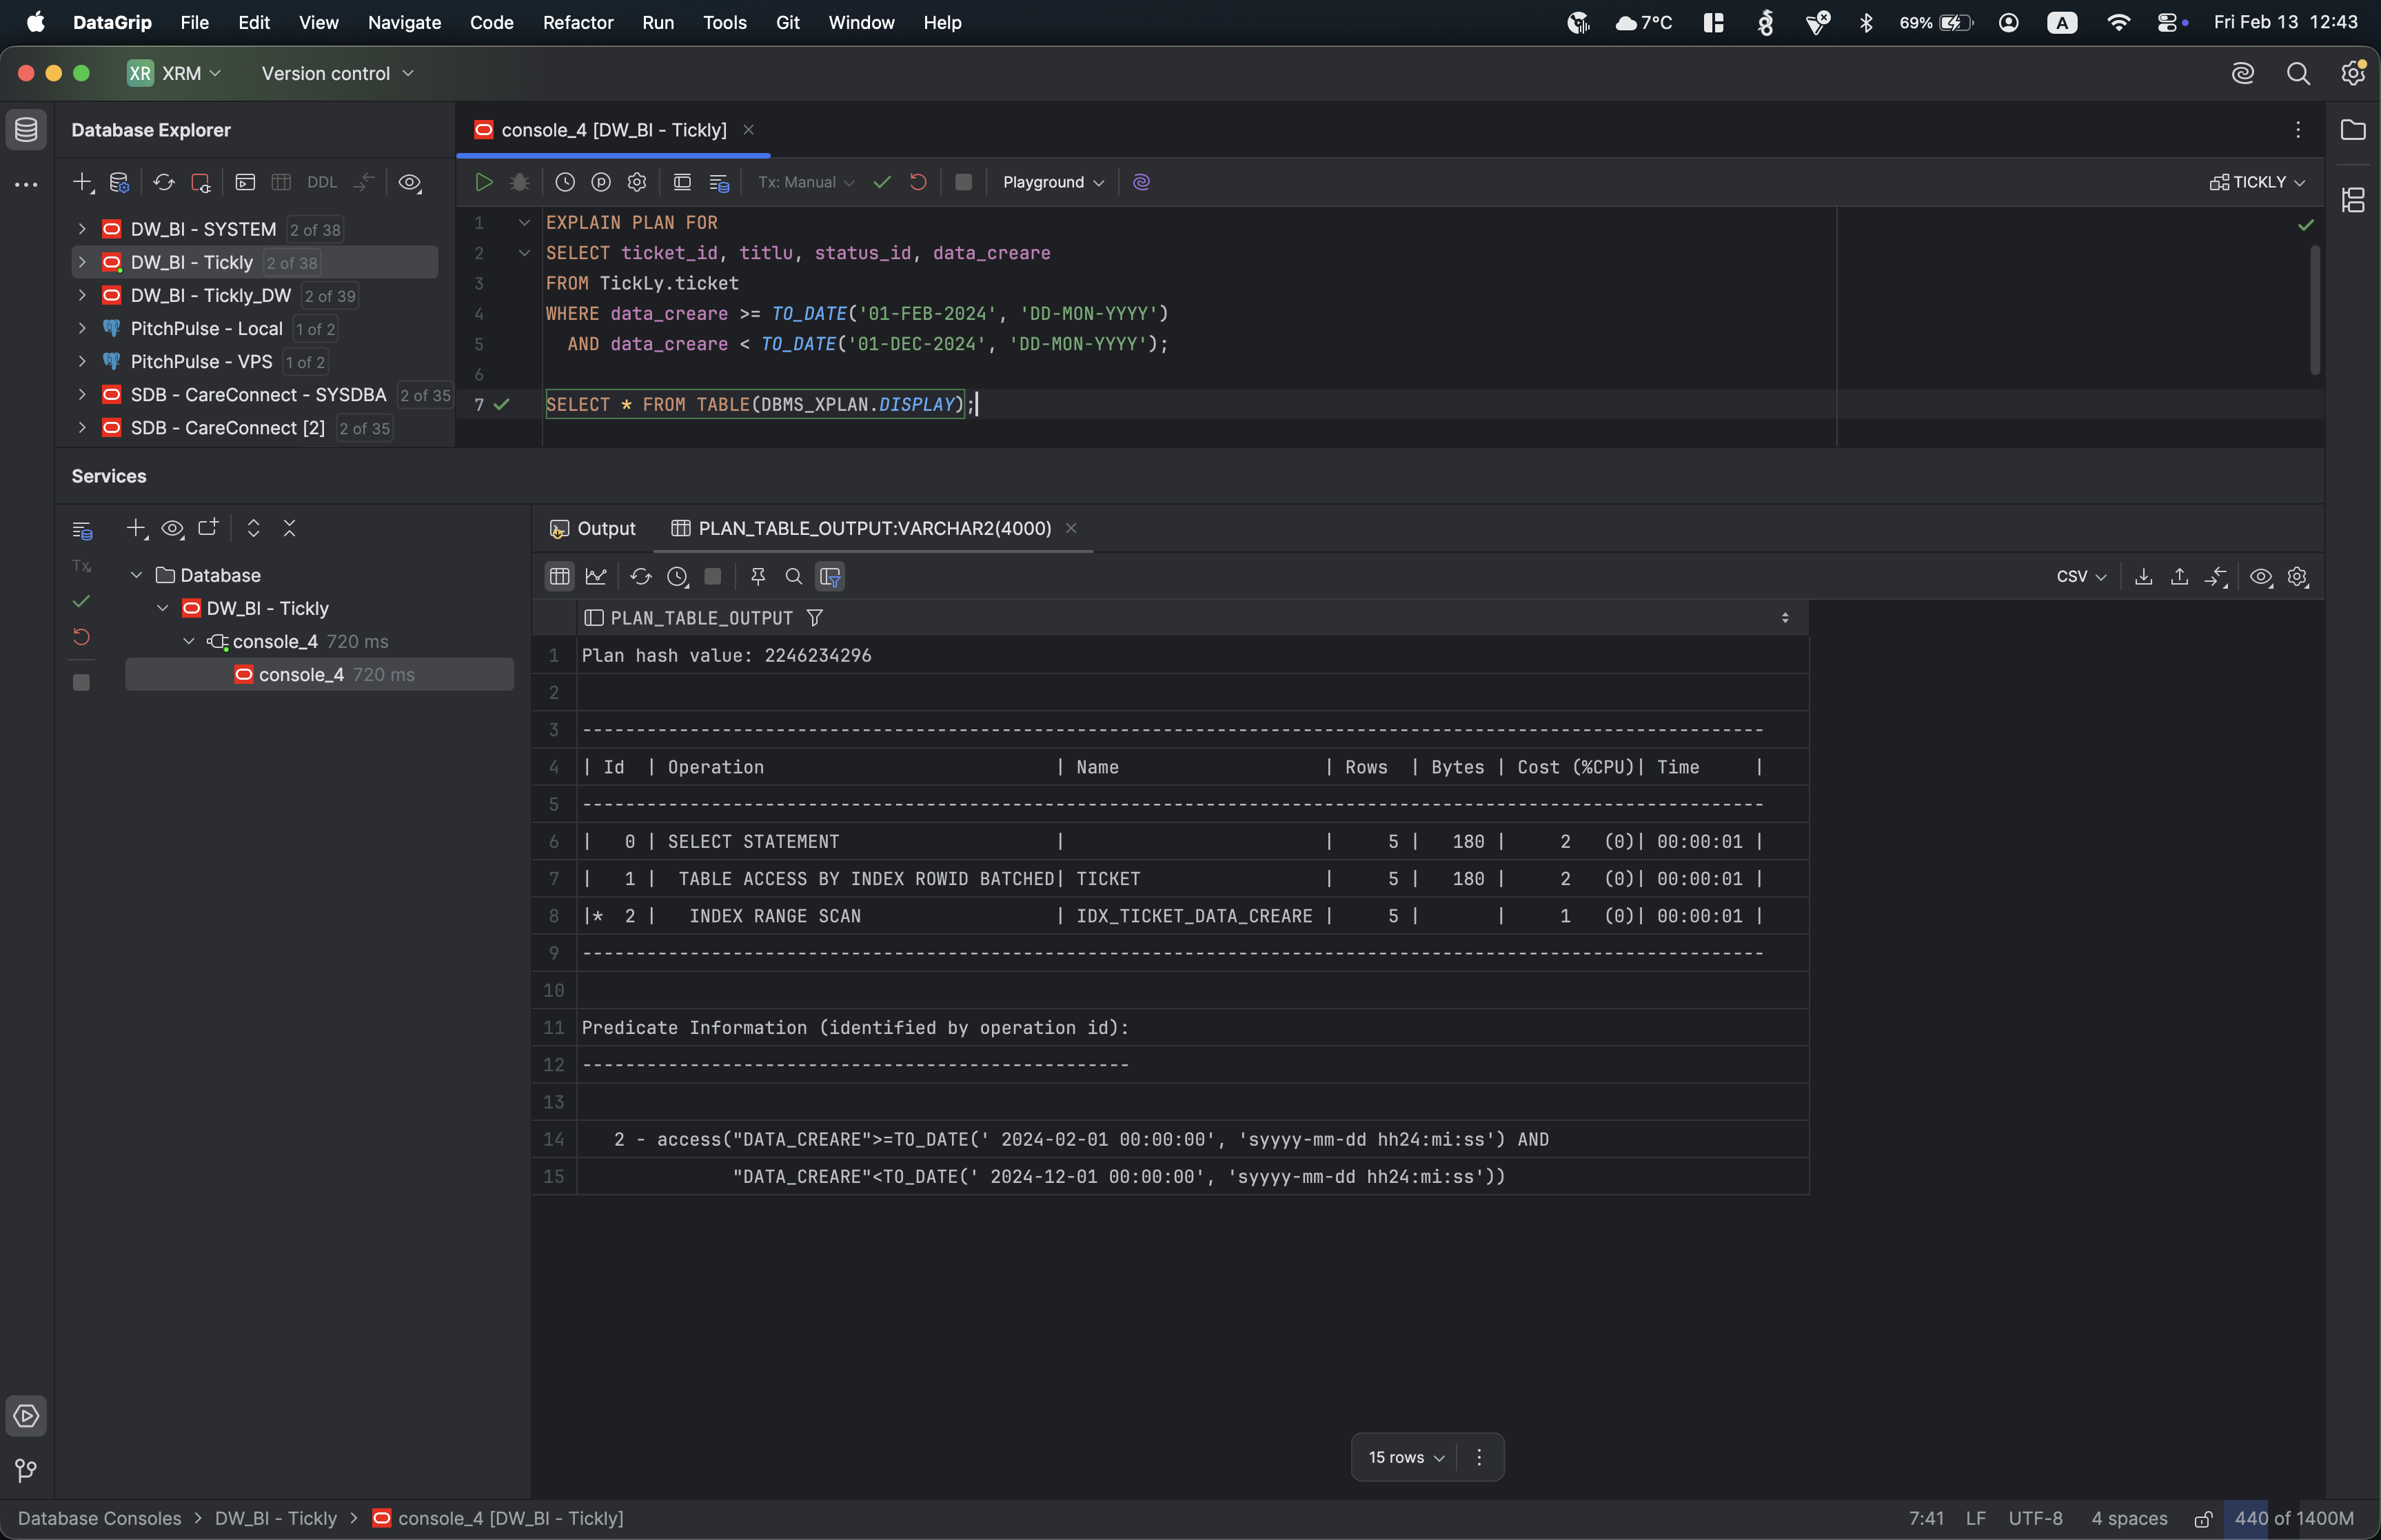
\includegraphics[width=0.6\textwidth]{../../scripts/tests/assets/oltp_date_index_explain.png}
        \caption{Plan de execuție query 2}
        \label{fig:plan_executie_query_2}
    \end{figure}

    \item \textbf{Depozit — indecși bitmap pe \texttt{fact\_ticket}}
    \begin{itemize}
        \item \textbf{3:} „Să se afișeze identificatorul din OLAP, cheia clientului și timpul de rezolvare (în ore) pentru tichetele care au un anumit status și/sau o anumită prioritate.”
    \end{itemize}

    \begin{figure}[H]
        \centering
        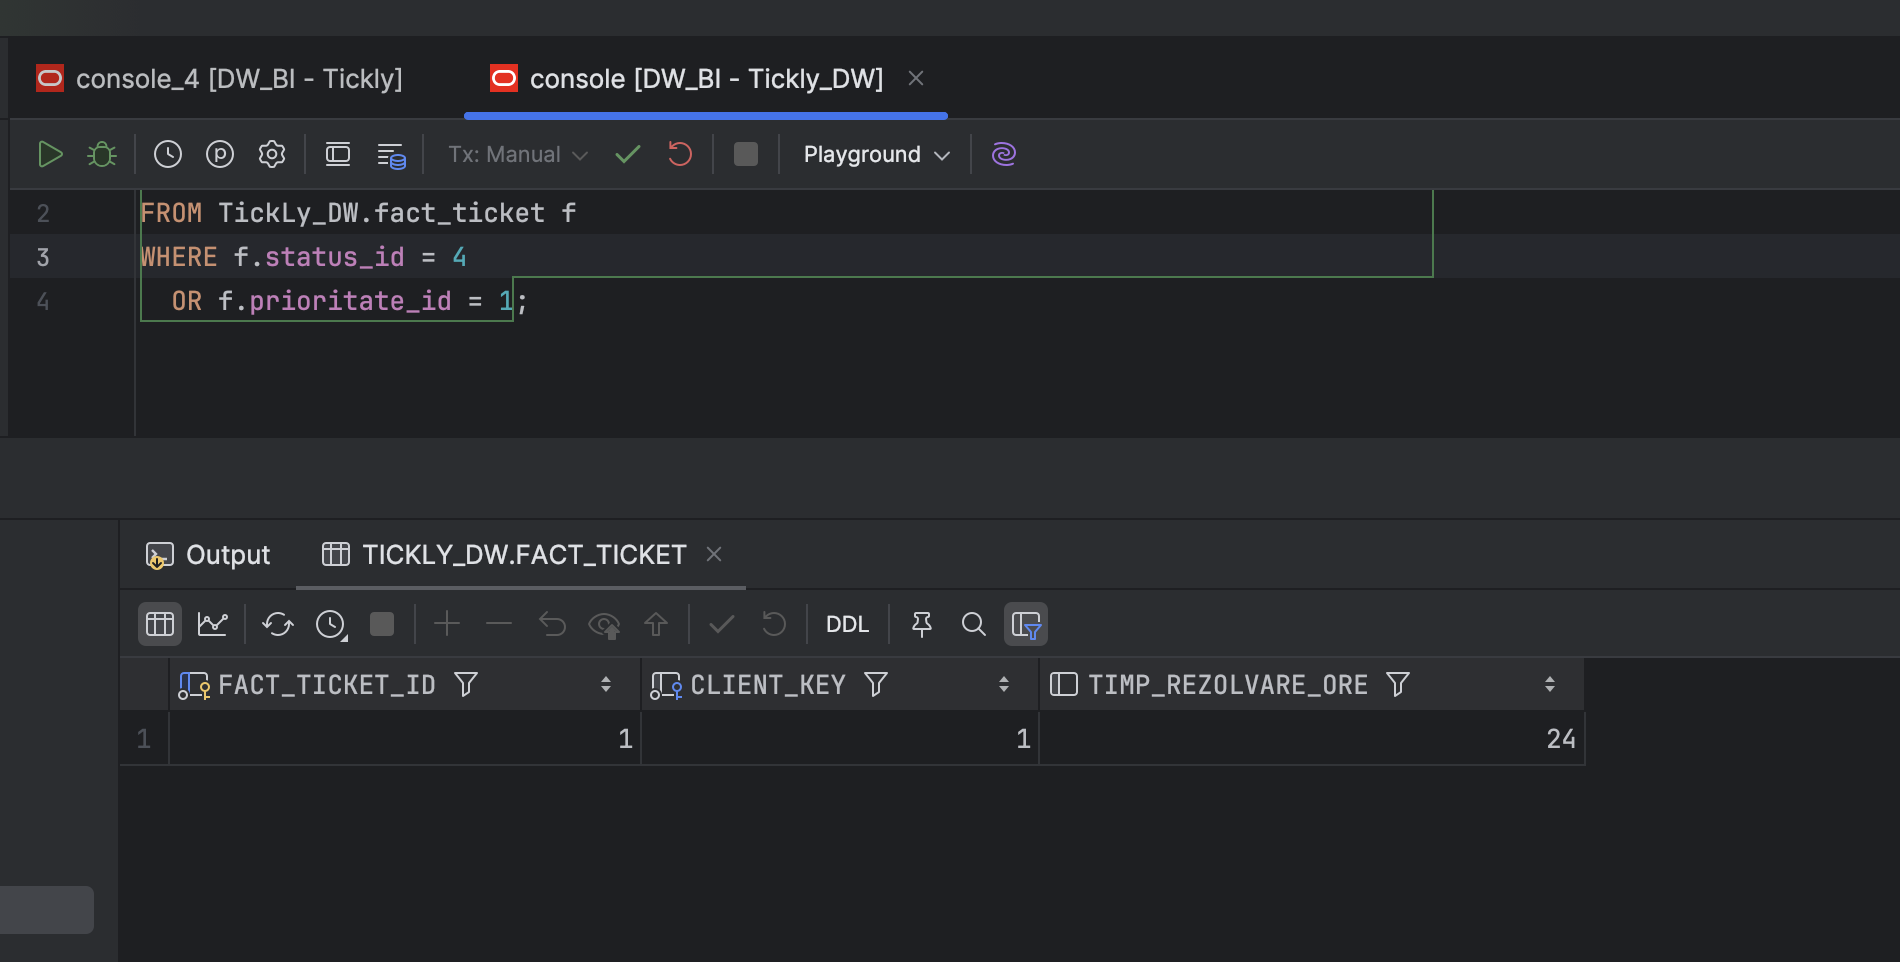
\includegraphics[width=0.6\textwidth]{./assets/indexes/test_3.png}
        \caption{Rulare query 3}
        \label{fig:rulare_query_3}
    \end{figure}

    \begin{figure}[H]
        \centering
        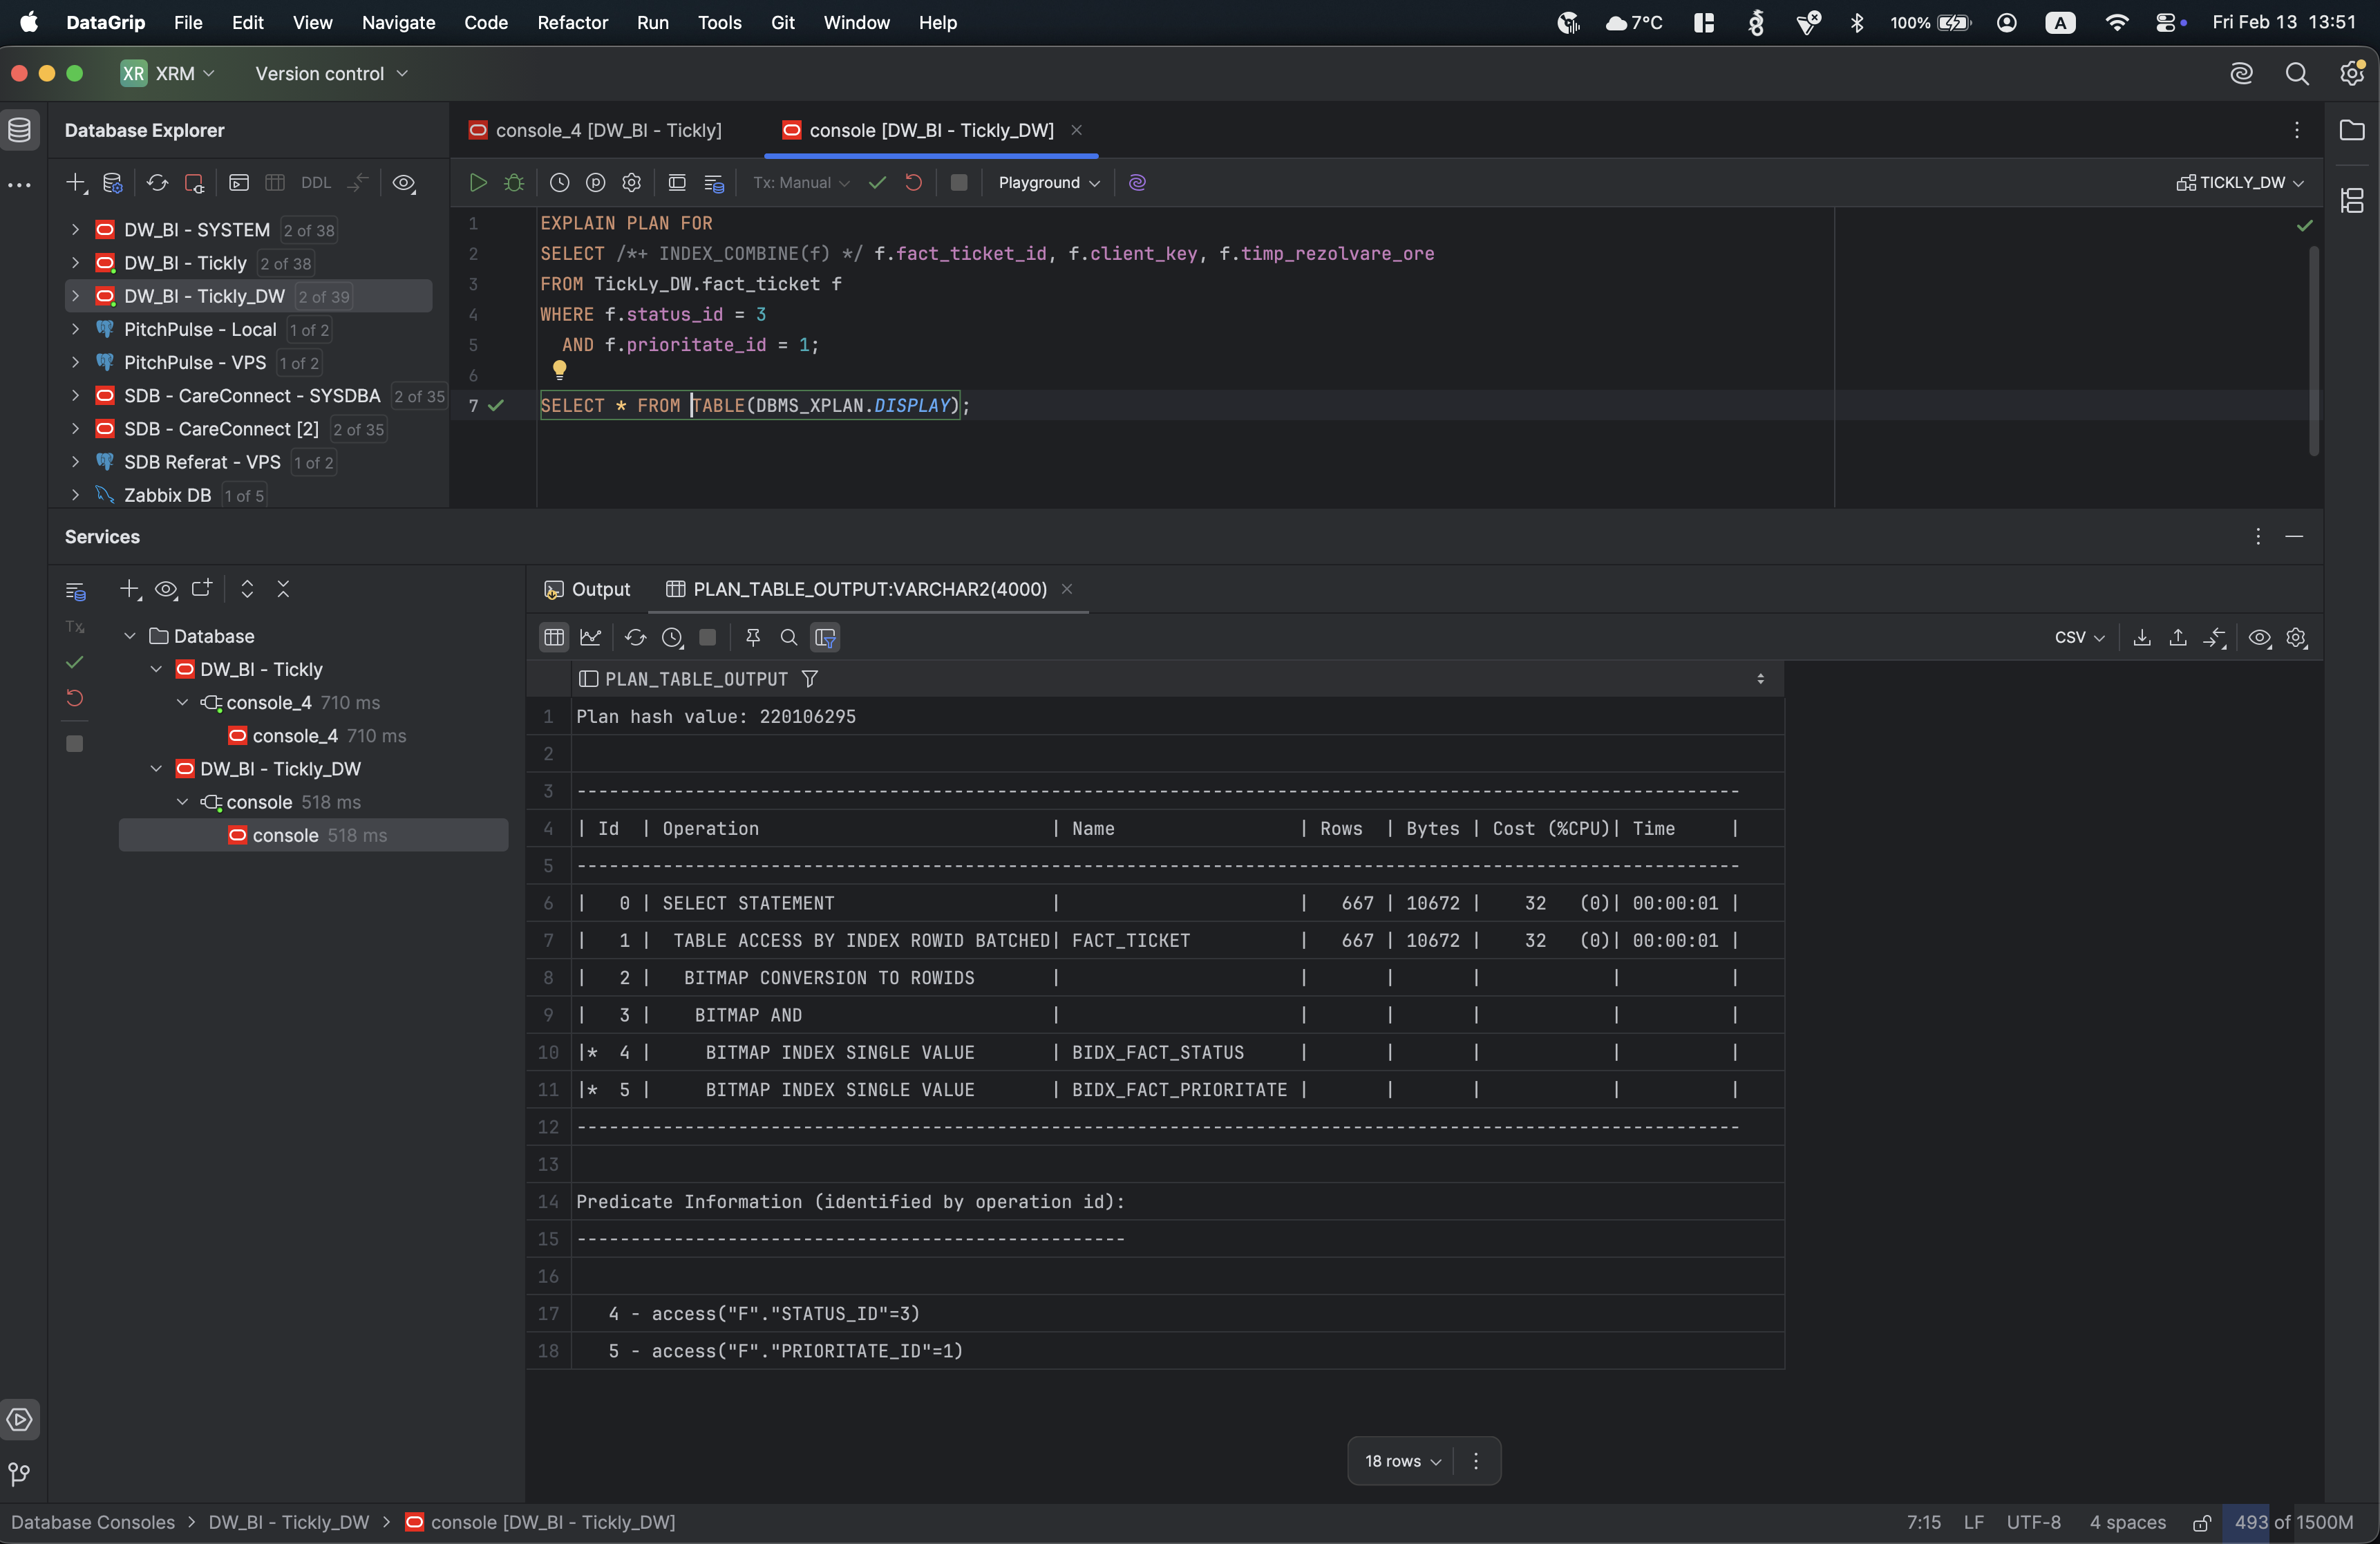
\includegraphics[width=0.6\textwidth]{../../scripts/tests/assets/olap_status_prio_explain.png}
        \caption{Plan de execuție query 3}
        \label{fig:plan_executie_query_3}
    \end{figure}

\end{enumerate}
